\documentclass{article}
\usepackage{amsmath}
\usepackage{amssymb}
\usepackage{graphicx}
\usepackage{fullpage}
\usepackage[parfill]{parskip}
\usepackage{tikz}
\usetikzlibrary{arrows, shapes}
\usepackage{pythonhighlight}
\newcommand{\pd}[2]{\frac{\partial #1}{\partial #2}}
\title{CS224n}
\author{Thomas Lu}
\date{}
\begin{document}
\maketitle
Note: statements that I am unsure about are enclosed in double square brackets, e.g. [[Every even integer greater than 4 can be expressed as the sum of two primes.]]
\section{Lecture 1: Introduction}
This lecture basically just gives a high level overview of the fields of Natural Language Processing (NLP) and Deep Learning (DL). Some highlights from the lecture:
\begin{itemize}
\item NLP is a study that aims for computers to understand natural (human) language well enough to perform useful tasks.
\item NLP has a lot of useful applications (virtual assistant, customer support automation, etc.) and has taken off commercially in the past few years.
\item What is special about NLP (vs. other subfields of ML)?
\begin{itemize}
\item Language is specifically constructed to convey information. It's not an environmental signal (e.g. an Amazon purchase, which I probably made for a reason other than conveying information).
\item Language is (mostly) a discrete/symbolic/categorical system, but our brains, which process language, are continuous systems.
\end{itemize}
\item What is special about DL (vs. other ML techniques)?
\begin{itemize}
\item Traditionally, learning an ML model requires an engineer/researcher to design and build relatively human-interpretable features. The machine then basically does some numerical optimization on these features to produce something useful. Note that this still requires a lot of intuitive human work to interpret data and figure out what parts of it might be useful.
\item In contrast, deep learning just feeds ``raw data" or very simplistic representations of data to a deep neural net, which then learns its own effective representations of the data, obviating the need for feature engineering.
\item DL has performed very well recently, e.g. speech recognition, ImageNet.
\end{itemize}
\item Why is NLP hard?
\begin{itemize}
\item Human language contains lots of contextual information. The meaning of a sentence may depend on something that was said a few sentences ago, a piece of information from another document, current events, or something observable in the environment (``Did you see that dog?" refers presumably to a dog in the speaker's field of vision).
\item Human language is also ambiguous by design; since speech is pretty slow at transmitting information, people will almost always leave ``relatively obvious" things unsaid in order to improve communication efficiency. Listeners are expected to infer these things. This is very different from computer languages, which must specify every posibility.
\end{itemize}
\end{itemize}

\section{Lecture 2: word2vec}
One part of NLP is word meaning representation. How do we represent the definition of a word so that a computer can do something useful with that representation?

One method is WordNet, which is a database of words that groups words with similar meaning together into synsets, which are also arranged in a kind of hierarchy. But this has some problems:
\begin{itemize}
\item Synonym/hypernym relationships miss a lot of nuance (e.g. ``expert", ``proficient", ``good" don't really mean the same thing).
\item It's hard to keep the database up-to-date when new words are added or existing words gain/lose usages and meanings.
\item Creating the database is subjective and labor-intensive.
\item Given two words, there isn't a good way to get a measure of how similar they are.
\end{itemize}
This is an example of a discrete/categorical/symbolic representation of words, where each word represents a single concept. Words might be related, but separate words are generally regarded as separate entities. If these words were vectors, each one would be a $V$-dimensional vector of zeroes with a single 1, where $V$ is the vocabulary size. This is sometimes referred to as a ``localist" or ``one-hot" representation.

A problem with these representations is that they lack similarity measures; we could try to manually encode some (as with WordNet), but they don't exist in the representations themselves (e.g. any two distinct word vectors are orthogonal). We can instead try to encode words so that they include similarity information, where a dot product of two words can give you a measure of their similarity. This gives us representations of words as shorter vectors, and this is known as a ``distributed" representation: instead of the meaning of a word being ``localized" to a single component of a vector, it's ``distributed" across multiple components.

One idea for generating distributed representations is the idea of distributional similarity, where we figure out the meaning of a word based on the contexts it appears in, i.e. its distribution in text. (The word ``distributional" in ``distributional similarity" is not related to the word ``distributed" in ``distributed representation".) This idea is summed up in a well-known quote: ``You shall know a word by the company it keeps." (John Rupert Firth)

word2vec is a well-known distributed representation model. Its key idea is to predict \textbf{outer words} that will appear in the context of a \textbf{center word}. More specifically, given a center word $w_c$, it attempts to predict the probabilities $p(w_o | w_c)$ that various outer words $w_o$ will appear in the context of $w_c$. Supposing we have a training corpus of $T$ words, the training process will attempt to maximize
$$\prod_{t=1}^T\prod_{\substack{-m \le j \le m,\\ j \ne 0}}p(w_{t+j} | w_t; \theta),$$
where $\theta$ is the parametrization of the model, the context of a word is defined as the $m$ words before and after it, $w_i$ is the $i$-th word in the corpus, and $p(w_i | w_j; \theta)$ denotes the model's predicted probability of $w_i$ appearing in the context of $w_j$ given its parametrization $\theta$. Equivalently, the training process attempts to minimize the objective function
$$J(\theta) = -\sum_{t=1}^T\sum_{\substack{-m \le j \le m,\\ j \ne 0}} \log p(w_{t+j} | w_t; \theta).$$
An example of a model trained in this way is the skip-gram word2vec model. This model is parametrized by $2|V|$ word vectors, where $V$ is the vocabulary. Each word $w \in V$ has two vector representations: a center word representation $v_w$ and an outer word representation $u_w$. The model then predicts
$$p(o | c) = \frac{\exp\left(u_o^T v_c\right)}{\sum_{w \in V} \exp\left(u_w^T v_c\right)}.$$
More intuitively, this means that the model predicts that $o$ is likely to appear in the context of $c$ if the outer word representation of $o$ is similar to the center word representation of $c$.

Because the training corpus for a word2vec model is typically very large, the model is usually trained using stochastic gradient descent, regarding each context window as a single training example. Now the gradient of $J$ with respect to $\theta$ is a little tricky to notate, but since $J$ is just a sum of terms of the form $\log p(w_o | w_c)$, the partial derivatives of that term will be quite informative. We have:
\begin{align*}
\frac{\partial}{\partial u_o} \log p(o | c) &= \frac{\partial}{\partial u_o} \log \frac{\exp\left(u_o^T v_c\right)}{\sum_{w \in V} \exp\left(u_w^T v_c\right)} \\
&= \frac{\partial}{\partial u_o} \left[ \log \exp\left(u_o^T v_c\right) - \log \left(\sum_{w \in V} \exp \left(u_w^T v_c\right)\right) \right]\\
&= v_c - \frac{1}{\sum_{w \in V} \exp \left(u_w^T v_c\right)} \frac{\partial}{\partial u_o} \sum_{w \in V} \exp \left(u_w^T v_c\right)\\
&= v_c - \frac{1}{\sum_{w \in V} \exp \left(u_w^T v_c\right)} \frac{\partial}{\partial u_o} \exp \left(u_o^T v_c\right)\\
&= v_c - \frac{\exp \left(u_o^T v_c\right)}{\sum_{w \in V} \exp \left(u_w^T v_c\right)} v_c \\
&= v_c\left(1 - p(o | c)\right)~.
\end{align*}
Similarly, we can calculate
\begin{align*}
\frac{\partial}{\partial v_c} \log p(o | c) &= \frac{\partial}{\partial v_c} \log \frac{\exp\left(u_o^T v_c\right)}{\sum_{w \in V} \exp\left(u_w^T v_c\right)} \\
&= \frac{\partial}{\partial v_c} \left[ \log \exp\left(u_o^T v_c\right) - \log \left(\sum_{w \in V} \exp \left(u_w^T v_c\right)\right) \right]\\
&= u_o - \frac{1}{\sum_{w \in V} \exp \left(u_w^T v_c\right)} \frac{\partial}{\partial v_c} \sum_{w \in V}\exp \left(u_w^T v_c\right)\\
&= u_o - \sum_{w \in V} \frac{\exp\left(u_w^T v_c\right)}{\sum_{w' \in V} \exp\left(u_{w'}^T v_c\right)} u_w\\
&= u_o - \sum_{w \in V} p(w | c)u_w \\
&= u_o\left(1 - p(o | c)\right) - \sum_{\substack{w \in V\\ w \ne o}}p(w | c)u_w~.
\end{align*}
Intuitively, this means that when we encounter a word $o$ in the context of another word $c$, we should:
\begin{itemize}
\item Move the outer word representation $u_o$ of $o$ towards the center word representation $v_c$ of $c$ by an amount negatively correlated with the prior prediction $p(o | c)$. This means that we should make a larger update for more unexpected events.
\item Move the center word representation $v_c$ of $c$:
\begin{itemize}
\item towards the outer word representation $u_o$ of $o$ by an amount negatively correlated with the prior prediction $p(o | c)$, meaning that we should make a larger update for more unexpected events; and
\item away from the outer word representations $u_w$ for each $w \in V \setminus \{w\}$ by an amount positively correlated with the prior prediction $p(w | c)$, meaning that we should make a larger update for more unexpected events (since observing $o$ in the context of $c$ means that we did not observe $w$ in the same location in the context of $c$.).
\end{itemize}
\end{itemize}
This matches our intuition that we expect to see $o$ in the context of $c$ if $u_o$ is similar to $v_c$.

\section{Lecture 3: GloVe}
\subsection{word2vec revisited}
Recall that the skip-gram word2vec model is typically trained using stochastic gradient descent. Because the parametrization of the model is very large ($2Vd$ terms, where $V$ is the vocabulary size and $d$ is the dimensionality of the vector representations of the words) and the calculated gradient at each iteration is comparatively sparse, we should avoid computing and passing around complete gradient vectors when performing SGD.

Previously, we used the following probability in the skip-gram model:
$$p(o|c) = \frac{\exp\left(u_o^T v_c\right)}{\sum_{w\in V}\exp\left(u_w^T v_c\right)}.$$
The numerator of this is easy to compute, but the denominator is pretty expensive, as the sum has to be taken across the entire vocabulary. Instead of computing the full sum, the actual skip-gram model uses a slightly different objective function that allows it to randomly sample from the vocabulary instead of iterating over the whole vocabulary:
$$J(\theta) = \sum_{t=1}^T J_t(\theta) = \sum_{t=1}^T \left[\log \sigma\left(u_o^T v_c\right) + \sum_{\substack{j\sim P(V)\\ k~\text{samples}}} \log \sigma\left(-u_j^T v_c\right)\right],$$
where $T$ represents our corpus, $\sigma$ is the sigmoid function, $\sigma(z) = (1 + e^{-z})^{-1}$, $P(V)$ is a probability distribution over the vocabulary $V$, $\sim$ indicates random sampling, and $k$ is a constant, usually around 10. Furthermore, instead of minimizing this objective function, the model actually seeks to maximize it. Intuitively, this means that the model attempts to maximize $u_o^T v_c$ when $o$ occurs in the context of $c$ and minimize $u_w^T v_c$ for $w$ that do not appear in the context of $c$, which is pretty similar to what we were doing with the previous objective function.

One detail on the objective function: the probability distribution $P(V)$ that is usually used is $P(w) = U(w)^{3/4}/Z$, where $U(w)$ is the unigram frequency of $w \in V$ and $Z$ is a normalizing factor to make $\sum_{w \in V} P(w) = 1$. The exponent of 3/4 ``smoothes out" the distribution a bit, so that more frequent items are less likely to be selected than less frequent items in proportion to their frequencies.

An alternative to the skip-gram model is the similar Continuous Bag-Of-Words (CBOW) model. While the skip-gram model attempts to predict the probability of an outside word appearing given a center word, the CBOW model attempts to predict the probability of the center word occuring given the sum of the (vector representation of the) outside words.

\subsection{Co-occurrence matrices}
Co-occurrence matrices are another way to construct vector representations of words. To start, we can create a $|V| \times |V|$ matrix $X$ and iterate through our corpus, incrementing $X_ij$ every time we see $i, j \in V$ occurring together. We can define ``occurring together", or co-occurrence, in various ways. Some common ones are:
\begin{itemize}
\item Window-based co-occurrence. This is similar to what the skip-gram model does: we say that two words co-occur if one appears in a window around the other (e.g. the window from 8 words before to 8 words after).
\item {[[Full-document co-occurrence. Here we say that two words co-occur if they both appear in some document in our corpus.]]}
\item {[[Word-document co-occurrence. In this definition, we need to change our matrix $X$. We will still have a row for each word, but instead of having a column for each word as well, we have a column for each document in our corpus, and we say that a word and a document co-occur if the word appears in that document.]]}
\end{itemize}

It turns out that window-based co-occurrence allows us to represent both syntactic and semantic information in the vector representations, while [[full-document co-occurrence and word-document co-occurrence allow us to capture topics and perform Latent Semantic Analysis.]] Unless otherwise specified, further discussion in this section will be about window-based co-occurrence matrices.

These ``raw" co-occurrence matrices, however, are extremely storage intensive; a 100,000 word vocabulary would yield a matrix with 10 billion entries when using window-based co-occurrence. These matrices are also rather sparse, which negatively impacts the robustness of models trained on them. We can solve both of these problems by reducing the column space using singular value decomposition (SVD). Other improvements that we can make to this model include:
\begin{itemize}
\item To prevent stopwords from creating very spiky counts, we can cap frequency counts when assembling the pre-SVD matrix or ignore stopwords altogether.
\item We can weight co-occurrences; e.g. maybe we should weight the co-occurrence of two words more if they are adjacent rather than 5 words apart (e.g. by adding a larger or smaller increment to the corresponding entry in the pre-SVD co-occurrence matrix).
\end{itemize}
However, co-occurrence matries still have some issues:
\begin{itemize}
\item Adding words to the vocabulary is difficult - we have to grow both the row space and the column space.
\item SVD is an expensive operation; on an $m\times n$ matrix with $n < m$, it has runtime $O(mn^2)$.
\item The model only captures word similarity and doesn't really capture any additional patterns.
\item It's hard to make the model not give excessive significance to large counts.
\end{itemize}
On the other hand, co-occurrence matrices have some advantages as well:
\begin{itemize}
\item It's relatively fast to train.
\item It uses the statistics of the corpus efficiently - after a single training pass, we can perform whatever further transformation/analysis we want on the co-occurrence counts.
\end{itemize}

As for the skip-gram model:
\begin{itemize}
\item The representations it produces are often better suited for downstream tasks.
\item It captures patterns beyond just word similarity - it also gets things like syntactical relationships.
\item The training time scales with the corpus size. It can take a very long time to train on a large corpus.
\item It doesn't really let us use corpus statistics well, as there isn't really any intermediate representation of the data besides the trained model itself.
\end{itemize}

\subsection{GloVe}
Global Vectors, or GloVe, is another method for training vector representations of words. It compiles a co-occurrence matrix $P$, and then seeks to minimize the objective function
$$J(\theta) = \frac{1}{2} \sum_{i, j \in V}f(P_{ij})\left(u_i^T v_j - \log P_{ij}\right)^2.$$
$f$ here is a function that is increasing until a cutoff point, after which it becomes constant. The parameters of the model here are the word vectors $u_i$ and $v_j$, similar to the skip-gram model.

Intuitively, we weight common co-occurrences more heavily in this objective function, but we have a cap on how heavily any one can be weighted. We also want $u_i^T v_j$ to be larger, i.e. $u_i$ and $v_j$ to be more similar, when $P_{ij}$ is larger (i.e. when $i$ and $j$ co-occur more frequently). At the end when we've trained our $u_i$ and $v_j$, the final representation $x_w$ that we choose for each word $w \in V$ is simply $x_w = u_w + v_w$.

This method scales to large corpora but has been shown to also work well for small corpora. It's like a best-of-both-worlds between word2vec and co-occurrence matrices: it's fast to train and uses statistics efficiently, but also captures information beyond word similarity and caps the influence of large co-occurrence counts. Furthermore, it avoids the computational cost of performing SVD on a large matrix.

\subsection{Evaluation of vector representations of words}
Once we have a model, we'd like to evaluate how well it performs. In general, there are two categories of evaluation metrics for any model: intrinsic and extrinsic.
\begin{itemize}
\item Intrinsic metrics measure how well the model performs some specific or intermediate subtask, such as how well vector similarities of words map to human judgments of similarities of words. They:
\begin{itemize}
\item are typically easy to compute and measure and
\item often can give you more insight into your own system by showing you which hyperparameters affect your system, but
\item oftentimes don't clearly show whether the model is actually good at some more externally useful task.
\end{itemize}
\item Extrinsic metrics measure how well the model performs some more useful downstream task, such as machine translation. Extrinsic metrics:
\begin{itemize}
\item are often slow to compute (e.g. it might take a while to train the machine translation model from your word representations) and
\item can be unclear on whether your component (e.g. word representations) of the larger system (e.g. machine translation system) specifically improved performance on its own if other parts of the system have also changed.
\end{itemize}
\end{itemize}
One intrinsic metric is word vector analogy accuracy. For example, if we give the analogy task\\
\centerline{\texttt{Paris:France::Rome:??}}
to the model, the model should be able to determine that the correct answer is Italy. Typically word representation models do this by finding the word $w$ that maximizes
$$\frac{(x_b - x_a + x_c)^T x_w}{||x_b - x_a + x_c||||x_w||},$$
where the analogy is given as \texttt{a:b::c:???}. We can then measure how well the model works by feeding it many such analogies and examining how many it gets correct.

\section{Lecture 4: Word Window Classification and Neural Networks}
Previously we have discussed unsupervised models for learning word representations, but eventually we want to use these representations to train supervised predictive models.

In a typical classification problem, we'll have a training dataset $(x_i, y_i), 1 \le i \le N$, where the $x_i$ are our inputs and the $y_i$ are labels that we want to train our model to predict. A legacy technique for training these models is logistic regression, a.k.a. softmax. In this method, we train a weight matrix $W$ with one row per class, and then attempt to adjust it so that our predictions
$$p(y|x) = \frac{\exp\left(W_y x\right)}{\sum_c \exp \left(W_c x\right)}$$
match the training examples as closely as possible. Here $W_c$ represents the row of weights in $W$ corresponding to the specific class $c$. A common loss function for softmax is the cross-entropy loss:
$$J(\theta) = \frac{1}{N} \sum_{i=1}^N -\log\frac{\exp \left( W_{y_i} x_i \right)}{\sum_c \exp\left(W_c x_i\right)},$$
where $\theta$ represents all the parameters of the model (in this case $W$). Oftentimes in practice we also add a regularization term $\lambda \theta^T \theta$, which helps prevent overfitting. Note that this method treats the inputs $X = [x_1^T, x_2^T, ..., X_N^T]^T$ as constant. In constrast, when we use deep learning models, we usually update our word vectors (i.e. $X$) as well. However, because this vastly increases our parameter space, we need to be careful not to overfit. Often if we have a small training set, we shouldn't update word vectors, as overfitting would be a big problem.

\subsection{Tips for vector calculus}
There will be a lot of vector calculus involved in calculating gradients for neural network (NN) models. Some tips for when it gets tricky:
\begin{itemize}
\item Carefully define all variables and keep track of their dimensionality. Checking dimensionality is a great sanity check for whether you've made any obvious mistakes.
\item When using the chain rule, keep track of variable dependencies to make sure you haven't forgotten a necessary step of differentiation.
\item Casework can sometimes make a calculation more intuitive (e.g. gradients for the correct class vs. the incorrect classes).
\item It can sometimes also be easier to calculate derivatives element-by-element instead of trying to differentiate the whole vector function at once.
\item After doing casework and elementwise differentiation, try to vectorize your notation again. It's important to vectorize your implementations in code, so you'll need to vectorize the notation at some point.
\end{itemize}

\subsection{Window classification}
A common prediction task is to predict whether a center word in a window of words is a named person/place/organization or not a named entity. Typically the input to the model is the concatenation of the word vectors in the window (so if we had $d$-dimensional word vectors and used a window with $m$ words before and after the center word, our input would be a vector of dimensionality $(2m + 1)d$). 

We could approach this problem with the softmax technique, but softmax is only capable of learning linear decision boundaries. NNs, on the other hand, can learn more complex nonlinear boundaries.

\subsection{Neural networks}
A neural network is made up of many neurons, arranged in sequential layers. We call the first layer the input layer, since it just contains the input values, and the final layer the output layer. The intermediate layers between them are commonly referred to as hidden layers. Each neuron has a weight vector $w$, an input vector $x$, a bias unit $b$, and an activation function $f$, and produces output $f(wx + b)$. A common activation function is the sigmoid function $f(z) = (1 + e^{-z})^{-1}$.

The reason that a neural network can learn more complex decision boundaries is that it can feed the outputs of neurons into another layer of neurons: instead of being constrained to immediately predict the output, it can learn an intermediate representation that might be more helpful for predicting the output. Note however that this requires a nonlinear activation function like the sigmoid; if we had a linear activation function, like the identity function, our neural network would still just be a linear classifier at the end of the day.

Back to our example problem - imagine that we're using a simple one-hidden-layer NN to predict whether the center word in a window is a named entity location or not. We have an input layer $x_j$ which together with a weight matrix $W$ produces a hidden layer $a_i$, which finally produces a score $s$. For simplicity, we will use a simple model where $s$ is a linear score: $s = U^Ta$ for some weight vector $U$. We will use the max-margin loss function:
$$J = \max\left(0, 1 - s + s_c\right),$$
where $s$ is predicted score of a positive example (where the center word is a named location) and $s_c$ is the predicted score of a negative example (where the center word is not a named location). In practice, for a single positive example, we usually randomly sample some $s_c$ rather than computing the max over the whole training corpus. Intuitively, this loss function tries to find a decision boundary that separates positive and negative samples by a ``sufficiently large" margin (``sufficiently large" is defined here as 1, but it can be tuned as a hyperparameter).

Note that it is very common to write $a = f(z)$, so that $a = f(Wx + b)$ and $z = Wx + b$. (Here $f$ is evaluated element-wise on each element of $z$.)

We now compute the gradient of $J$ in parts. When $J = 0$ we have $\vec{\nabla} J = 0$, so assume $J > 0$. Then $\vec{\nabla} J = -\vec{\nabla}s + \vec{\nabla}s_c$. We will just compute $\vec{\nabla}s$ for illustration. For the partial derivatives with respect to $U$, we have:
$$\frac{\partial s}{\partial U} = \frac{\partial}{\partial U} U^Ta = a.$$
For the partial derivatives with respect to $W$, we have:
$$\frac{\partial s}{\partial W_{ij}} = \frac{\partial}{\partial W_{ij}} U^Ta = \frac{\partial}{\partial W_{ij}}U^Tf(z) = \frac{\partial}{\partial W_{ij}} U^Tf(Wx + b).$$
Note that only the $i$-th entry of $f(Wx + b)$ is nonconstant with respect to $W_{ij}$, so we have
\begin{align*}
\frac{\partial}{\partial W_{ij}} U^Tf(Wx + b) &= \frac{\partial}{\partial W_{ij}} U_if(W_ix + b_i)\\
&= U_if'(z_i)x_j\\
&= \delta_ix_j,
\end{align*}
where we have written $\delta_i = U_if'(z_i)$. Now note that by combining all of these entries, we can write:
$$\frac{\partial s}{\partial W} = \delta x^T.$$
To calculate the partials with respect to $b$, we have:
\begin{align*}
\frac{\partial s}{\partial b_i} &= \frac{\partial}{\partial b_i}U^Tf(Wx + b) = \frac{\partial}{\partial b_i} U_if(W_ix + b_i)\\
&= U_if'(W_ix + b_i)\\
&= \delta_i\\
\Rightarrow \frac{\partial s}{\partial b} &= \delta.
\end{align*}
Finally it remains to find the partials with respect to $x$. We have:
\begin{align*}
\frac{\partial s}{\partial x_j} &= \frac{\partial}{\partial x_j} U^Ta \\
&= \sum_i \frac{\partial}{\partial x_j} U_ia_i\\
&= \sum_i U_i\frac{\partial}{\partial x_j} f(W_ix + b_i)\\
&= \sum_i U_i f'(W_ix + b_i) \frac{\partial}{\partial x_j} W_ix\\
&= \sum_i \delta_iW_{ij}\\
\Rightarrow \frac{\partial s}{\partial x} &= W^T\delta.
\end{align*}

\section{Lecture 5: Backpropagation}
Let's now imagine a neural network with two hidden layers, still using the same output layer and cost function as before. We now have:
$$s = U^Ta^{(3)}$$ 
\begin{align*}
&a^{(3)} = f(z^{(3)}) &z^{(3)} = W{(2)}a^{(2)} + b^{(2)}\\
&a^{(2)} = f(z^{(2)}) &z^{(2)} = W^{(1)}x + b^{(1)}\\
\end{align*}
We can easily derive $s$ with respect to $U$ and $W^{(2)}$ just as we did before to get
\begin{align*}
\frac{\partial s}{\partial U} &= a^{(3)} \\
\frac{\partial s}{\partial W^{(2)}} &= \delta^{(3)}a^{(3)T},
\end{align*}
where $\delta^{(3)} = U \circ f'(z^{(3)})$, with $\circ$ denoting the element-wise product of two vectors. We can calculate $\partial s/\partial b^{(2)} = \delta^{(3)}$ similarly as well.

It now remains to calculate the partials of $s$ with respect to $W^{(1)}$, $b^{(1)}$, and $x$. We will demonstrate the computation for $W^{(1)}$:
\begin{align*}
\frac{\partial s}{\partial W_{ij}^{(1)}} &= \frac{\partial}{\partial W_{ij}^{(1)}}U^Tf(W^{(2)}a^{(2)} + b^{(2)})\\
&= \sum_k\frac{\partial}{\partial W_{ij}^{(1)}} \left[U_k f(W_k^{(2)}a^{(2)} + b_k^{(2)}) \right]\\
&= \sum_k  U_kf'(W_k^{(2)}a^{(2)} + b_k^{(2)}) \frac{\partial}{\partial W_{ij}^{(1)}} W_k^{(2)}a^{(2)}\\
&= \sum_k \delta^{(3)}_k \frac{\partial}{\partial W_{ij}^{(1)}}W_k^{(2)}f(W^{(1)}x + b^{(1)})\\
&= \sum_k \delta^{(3)}_k \frac{\partial}{\partial W_{ij}^{(1)}}W_{ki}^{(2)}f(W_i^{(1)}x + b_i^{(1)})\\
&= \sum_k \delta^{(3)}_k W_{ki}^{(2)} f'(W_i^{(1)}x + b_i^{(1)})\frac{\partial}{\partial W_{ij}^{(1)}} \left(W_i^{(1)}x + b_i^{(1)}\right)\\
&= \sum_k \delta_k^{(3)} W_{ki}^{(2)} f'(z^{(2)}_i)x_j\\
&= x_jf'(z_i^{(2)})\left(W_{.i}^{(2)T}\delta^{(3)}\right)\\
\Rightarrow \frac{\partial s}{\partial W^{(1)}} &= \left(f'(z^{(2)}) \left(\circ W^{(2)T} \delta^{(3)}\right)\right) x^T = \delta^{(2)} x^T,
\end{align*}
where
$$\delta^{(2)} = \left(W^{(2)T} \delta^{(3)}\right) \circ f'(z^{(2)}).$$
It's easy to see from the previous derivation that $\partial s/\partial b^{(1)} = \delta^{(2)}$, and the partial with respect to $x$ can be found in a similar way.

In general, we have
\begin{align*}
\delta^{(\ell)} &= \left(W^{(\ell)T}\delta^{(\ell + 1)}\right) \circ f'(z^{(\ell)})\\
\frac{\partial E_R}{\partial W^{(\ell)}} &= \delta^{(\ell + 1)}a^{(\ell)T} + \lambda W^{(\ell)},
\end{align*}
for any intermediate layer $\ell$, any activation function $f$, and regularization with constant $\lambda$.

\section{Lecture 6: Dependency Parsing}
Two main models of linguistic structure are used these days. 
\begin{itemize}
\item One is the constituency model, also commonly referred to as phrase structure grammar model or the context free grammar model. This attempts to organize words into nested constituents (noun phrase, verb phrase, prepositional phrase, etc.) and define how these constituents can be constructed (e.g. a noun phrase is a determinant, followed by an arbitrary number of optional adjectives, followed by a noun, folllowed by an arbitrary number of optional prepositional phrases).
\item The other is the dependency model, which the rest of this section will focus on. In this model, we typically just care about which words depend on (modify or are arguments of) which other words. Oftentimes dependency structures are depicted with dependency diagrams, in which dependencies between words in a sentence are indicated with arrows pointing from words to the words dependent on them.
\end{itemize}
Sometimes, the meaning of a sentence can be ambiguous, e.g. ``Scientists study whales from space." Ambiguities such as these often come from ambiguous dependency structures (does ``from space" depend on ``whales" or ``study"?).

To train sentence-parsing models using dependency structures, there are ``treebanks," which are datasets of dependency-annotated sentences. While intuitively it may seem advantageous for the field to spend time designing grammars instead of manually annotating sentences (grammars generalize, annotating sentences is very slow, etc.), it turns out that human-created grammars differ a lot and that the work involved in designing grammars isn't very reusable, while treebanks are highly reusable and provide a useful ground truth for future work.

In a dependency syntax, we represent sentences as directed graphs of words, where words are nodes and edges point from ``head" nodes to ``dependent" nodes (dependent nodes depend on head nodes). Edges are often also annotated with the type of dependence (e.g. auxiliary, case, subject, etc.). Normally, this graph is a tree: it has a single root, is acyclic, and is connected. Usually there will also be a pseudoword ROOT in the sentence so that every other word in the sentence depends on one word.

When evaluating the plausibility of a dependence from one word to another in a sentence, there are various information sources that we can draw from:
\begin{itemize}
\item Bilexical affinities (is it reasonable, based on the definitions of the word, for word A to depend on word B?)
\item Distance (words are generally more likely to depend on nearby words)
\item Intervening material (e.g. an adjective and the noun it's modifying are unlikely to have a verb between them)
\item Valency of heads (certain words are likely to have certain numbers of dependents on the left and/or right side; e.g. determinants are unlikely to have any dependents; nouns might have many dependents but determiners and adjectives typically are on the left, while prepositional phrases are likely to be on the right).
\end{itemize}

To parse a sentence, we must decide for each word which other word it depends on. Usually we constrain the total space of possibilities by enforcing that only one word depends on ROOT, and that dependencies cannot form cycles, which guarantees that our dependency graph will be a tree. We also say that a dependency graph is projective if, when we draw it with the words in order and all edges as ``straight" arcs (i.e. never change their left-right direction) going over the row of words, we can draw it in such a way that the arcs don't cross.

There are various methods for doing dependency parsing:
\begin{itemize}
\item Dynamic programming (runs in $O(n^3)$)
\item Graph algorithms (minimum spanning tree)
\item Constraint Satisfaction: eliminate edges that don't satisfy hard constraints
\item ``Transition-based parsing." Slightly less accurate than graph algorithms, but is a greedy algorithm that runs in linear time. This is what's most commonly used today.
\end{itemize}
\subsection{Arc-standard transition-based parser}
The arc-standard transition-based parser is one form of transition-based parsing (there are others). In this algorithm, we have a buffer $\beta$ that initially consists of all the words of the sentence in order from left to right, and a stack $\sigma$ that initially contains one element: ROOT. At each step, we have three operations that we can perform:
\begin{enumerate}
\item Shift. This pops the leftmost word from $\beta$ and pushes it onto $\sigma$.
\item Left Arc. This sets the second-from-the-top element of the stack as dependent on the top element of the stack and removes the second-from-the-top element.
\item Right Arc. The same as left arc, but the top element is the dependent instead of the head.
\end{enumerate}
As an example, we perform this algorithm on the simple sentence ``I ate fish." In this example, the right side of the stack is the top.
\begin{enumerate}
\item At the beginning, we have $\sigma = [\text{ROOT}], \beta = [\text{I}, \text{ate}, \text{fish}].$
\item We perform two shift operations, and now we have $\sigma = [\text{ROOT}, \text{I}, \text{ate}], \beta = [\text{fish}].$
\item We perform a left-arc, so now `I' depends on `ate' and is removed from $\sigma$, so we have $\sigma = [\text{ROOT}, \text{ate}], \beta = [\text{fish}].$
\item We now perform another shift, giving $\sigma = [\text{ROOT}, \text{ate}, \text{fish}]$, and $\beta$ is now empty.
\item We follow this up with a right-arc, so `fish' depends on `ate', and now $\sigma = [\text{ROOT}, \text{ate}].$
\item Finally, we perform another right-arc, and $\sigma = [\text{ROOT}]$, `ate' depends on ROOT, and `I' and `fish' depend on `ate'.
\end{enumerate}
To train a model to actually do this, we can use the a treebank - given the dependency structure, we can figure out which sequence of shifts and left/right-arcs will give us the correct structure. This allows us to train a classifier on which operation is correct at each step. In the model above, we have 3 possible operations at each step, but in practice we also want to label each dependency in a dependency structure with a type (i.e. not just that `fish' depends on `ate', but that it is specifically the object of `ate'). To accommodate this, we have a different left-arc and right-arc operation for each dependency type, giving $2R+1$ total distinct operations, where $R$ is the number of types of dependencies. These dependencies are often scored using two metrics: UAS, which counts the percentage of dependency arrows that are correct, and LAS, which counts the percentage of depdency arrows that are both correct \emph{and} correctly labeled.

These classifiers were commonly built with sparse feature representations at first, where we use binary vectors where an element is 1 if some specific position on either the stack or the buffer contains some specific word in some specific part of speech (e.g. `set' can be multiple parts of speech depending on context). However, you often end up with $O(10^7)$ features, which causes issues where there are too many possible configurations of features, some of which you will almost certainly never see in your training data. The vast feature space also makes for rather expensive computation.

So instead, we can learn a dense feature representation. We use $d$-dimensional distributed representations of words, and also smaller-dimensioned distributed representations of parts of speech. We can then extract features by looking at certain stack/buffer positions and concatenating the word/POS vectors. We can then learn on these features with a neural network; it turns out a single hidden layer with a ReLU activation function and an output layer with a softmax activation function works pretty well.

\section{Lecture 7: Intro to TensorFlow}
TensorFlow (TF) is a deep learning framework from Google. There are various reasons why these frameworks are useful:
\begin{itemize}
\item Provides simple ways to make ML code to run at massive scales
\item Compute gradients automatically
\item Standardizes ML so that work can be shared more easily
\item Allows easy interfacing with GPUs
\end{itemize}
The core idea of TF is that numerical computation is a graph, where nodes are operations, and they take inputs and transmit outputs via edges. In addition to ``normal" operations such as addition or matrix multiplication, there are also two important special types of operations:
\begin{itemize}
\item Variables, which output their current value. The current value is stored as state of the node. Gradient descent updates will also by default update all variables in the graph. Usually these will be the parameters of your model.
\item Placeholders, which are nodes whose values are fed in at execution time. Usually these will be the training inputs/labels of your model.
\end{itemize}
As an example, the equation $h = ReLU(Wx + b)$ (which could represent a one-layer neural network with a ReLU activation function) would be expressed as graph in Figure \ref{fig7-1}.
\begin{figure}
\centering
\begin{tikzpicture}[
    tfvar/.style={shape=circle, draw=black, minimum size=1cm},
    tfph/.style={shape=diamond, draw=black, minimum size=1cm},
    tfop/.style={shape=rectangle, draw=black, minimum width=3cm, minimum height=1cm},
]
\node[tfvar] (W) at (2, 0) {$W$};
\node[tfph] (x) at (6, 0) {$x$};
\node[tfvar] (b) at (0, 2) {$b$};
\node[tfop] (mul) at (4, 2) {MatMul};
\node[tfop] (add) at (4, 4) {Add};
\node[tfop] (relu) at (4, 6) {ReLU};

\path[->]
    (W) edge node {} (mul)
    (x) edge node {} (mul)
    (b) edge node {} (add)
    (mul) edge node {} (add)
    (add) edge node {} (relu)
;
\end{tikzpicture}
\caption{The expression $ReLU(Wx + b)$ as a TF computation graph.} \label{fig7-1}
\end{figure}
In code, this might be (assuming that we have 784-dimensional training examples in batches of 2000, and that our output is 100-dimensional):
\begin{python}
import tensorflow as tf

b = tf.Variable(tf.zeros((100,)))
W = tf.Variable(tf.random_uniform((100, 784), -1, 1))

x = tf.placeholder(tf.float32, (784, 2000))

h = tf.nn.relu(tf.matmul(x, W) + b)
\end{python}

Now to actually run this computation, we need to deploy it in a TF session, which binds to a particular execution context (e.g. CPU, GPU, TPU). When running a session, we need to provide two arguments:
\begin{itemize}
\item Fetches. This is the list of graph nodes whose values we care about. These will be returned by the \pyth{run} function.
\item Feeds. This maps graph nodes to specified concrete values, and e.g. allows us to specify the values of placeholders.
\end{itemize}
If we extend our code example from earlier to run the graph, it might look like this:
\begin{python}
import tensorflow as tf

b = tf.Variable(tf.zeros((100,)))
W = tf.Variable(tf.random_uniform((100, 784), -1, 1))

x = tf.placeholder(tf.float32, (784, 2000))

h = tf.nn.relu(tf.matmul(x, W) + b)

sess = tf.Session()
sess.run(tf.initialize_all_variables())
sess.run(h, {x: np.random.random(784, 2000)})
\end{python}
In the last line, \pyth{h} is our fetch and \pyth{x} is our feed. Here we're just initializing our training data randomly; in an actual application we'd probably load it in from somewhere. The \pyth{Session} constructor could optionally also take a computation environment as a function parameter. (There's probably other function parameters as well.)

We now need to define a loss function. To do this, we create a placeholder for the training labels and create a loss node using those and our prediction values:
\begin{python}
prediction = tf.nn.softmax(h)
label = tf.placeholder(tf.float32, [100, 2000])
# cross entropy per example
cross_entropy = -tf.reduce_sum(label * tf.log(prediction), axis=1)
\end{python}
Then to actually train the model, we need to perform gradient descent. We can use an Optimizer object, which allows us to add an optimization operation to our computation graph. For example, to perform gradient descent, we can do:
\begin{python}
train_step = tf.train.GradientDescentOptimizer(0.5).minimize(cross_entropy)
\end{python}
Here 0.5 is a learning rate, and \pyth{train_step} now refers to a optimization operation node. When we run \pyth{train_step} in a session, it does two things: it calculates the gradients with respect to the variables in the graph, and it also adjusts the values of the variables according to those gradients. TF is able to calculate these gradients because each graph node has an attached gradient operation, and the graph structure of the computation allows TF to easily apply the chain rule.

To tie this all together, our final code might look like this:
\begin{python}
import tensorflow as tf
from . import data  # some data loading code you defined

b = tf.Variable(tf.zeros((100,)))
W = tf.Variable(tf.random_uniform((100, 784), -1, 1))

x = tf.placeholder(tf.float32, (784, 2000))
h = tf.nn.relu(tf.matmul(x, W) + b)

prediction = tf.nn.softmax(h)
label = tf.placeholder(tf.float32, [100, 2000])
# cross entropy per example
cross_entropy = -tf.reduce_sum(label * tf.log(prediction), axis=1)

train_step = tf.train.GradientDescentOptimizer(0.5).minimize(cross_entropy)

for i in range(1000):  # train on 1000 batches
    batch_x, batch_label = data.next_batch()
    sess.run(
        train_step, 
        feed_dict={
            x: batch_x,
            label: batch_label
        }
    )
\end{python}

\subsection{Variable sharing}
Sometimes we want to use multiple machines to train our models, and we need to share variables between them. TF has a concept called variable sharing that allows us to do this. In TF, we can enter a variable scope using \pyth{with tf.variable_scope('foo')}, and within that scope, we can call \pyth{tf.get_variable('v')}.

We can use \pyth{get_variable} to create new variables or access the values of existing ones. Its exact behavior depends on the value of the \pyth{reuse} keyword argument passed to the enclosing \pyth{variable_scope} (details can be found on the official TF documentation).

\section{Lecture 8: Recurrent Neural Networks and Language Models}
A language model is a model that predicts the probability of a sequence of words: $p(w_1, w_2, \dots, w_T)$. Language models have applications in machine translation (e.g. $p(\text{the cat is small}) > p(\text{small is the cat}))$ and speed recognition (e.g. $p(\text{walking home after school}) > p(\text{walking hone after school}))$, among other things. 

\subsection{Traditional Language Models}
Traditional language models are typically set up so that the probability of a word is conditioned on a window of $n$ previous words. For reasons of computational complexity, $n$ is usually small; as $n$ increases, performance improves significantly, but the storage and training time requirements grow extremely quickly. Thus these models are pretty limited, since words in a language often depend on other words that occurred quite long ago.

In a traditional language model, if $n = 2$, we might estimate probabilities based on the last word and the last two words like so:
$$p(w_2 | w_1) = \frac{\text{count}(w_1w_2)}{\text{count}(w_1)}$$
$$p(w_3 | w_1, w_2) = \frac{\text{count}(w_1w_2w_3)}{\text{count}(w_1w_2)}$$

\subsection{Recurrent Neural Networks}
A recurrent neural network (RNN) is basically a neural network that produces an output at each time step $t$, and where the hidden layer at time $t-1$ feeds into the hidden layer at time $t$. Mathematically, suppose that we have a vocabulary $V$ and a corpus/document represented as a list of word vectors $x_{[1]}, x_{[2]}, \dots, x_{[t-1]}, x_{[t]}, x_{[t+1]}, \dots, x_{[T]}$. Then at each time step $t$, we perform:
\begin{itemize}
\item $h_t = \sigma(W^{(hh)}h_{t-1} + W^{(hx)}x_{[t]})$
\item $\hat{y}_t = \text{softmax}(W^{(S)}h_t)$
\item Predict $\hat{P}(x_{[t+1]} = v_j \in V | x_{[t]}, \dots, x_{[1]}) = \hat{y}_{t,j}$.
\end{itemize}
Here $W^{(hh)} \in \mathbb{R}^{D_h \times D_h}, W^{(hx)} \in \mathbb{R}^{D_h \times d}, W^{(S)} \in \mathbb{R}^{|V| \times D_h}$ are three separate weight matrices (shared across all time steps) that are used in different parts of the model. Sharing these weights between time steps effectively allows the model to ``remember" what happened more than a few words ago, so that we can build a more effective language model.

\begin{figure}
\centering
\begin{tikzpicture}[
    rnnstep/.style={shape=circle, draw=black, minimum size=1cm},
    rnnempty/.style={shape=circle, draw opacity=0, minimum size=1cm},
]

\node[rnnempty] (hm2) at (0, 2) {$\dots$};
\node[rnnempty] (ym1) at (2, 4) {$\vdots$};
\node[rnnempty] (xm1) at (2, 0) {$\vdots$};
\node[rnnstep] (hm1) at (2, 2) {$h_{t-1}$};
\node[rnnstep] (h0) at (4, 2) {$h_t$};
\node[rnnstep] (y0) at (4, 4) {$y_t$};
\node[rnnstep] (x0) at (4, 0) {$x_{[t]}$};
\node[rnnstep] (h1) at (6, 2) {$h_{t+1}$};
\node[rnnempty] (y1) at (6, 4) {$\vdots$};
\node[rnnempty] (x1) at (6, 0) {$\vdots$};
\node[rnnempty] (h2) at (8, 2) {$\dots$};

\path[->]
    (hm2) edge node {} (hm1)
    (xm1) edge node {} (hm1)
    (hm1) edge node {} (ym1)
    (hm1) edge node {} (h0)
    (x0) edge node {} (h0)
    (h0) edge node {} (y0)
    (h0) edge node {} (h1)
    (h1) edge node {} (y1)
    (x1) edge node {} (h1)
    (h1) edge node {} (h2)
;
\end{tikzpicture}
\caption{A common visualization of RNNs.}
\end{figure}

As a minor detail of implementation, we typically initialize $h_0$ to a vector of all zeros so that there is some defined starting value.

With this RNN, we can define a loss function. Since $\hat{y}_t$ gives us a probability distribution over $V$, we can calculate the cross entropy loss at each time step:
$$J^{(t)} = \sum_{j=1}^{|V|} y_{t,j} \log{\hat{y}_{t,j}}$$
After calculating these, we typically use perplexity as a loss function (lower is better):
$$E = \text{perplexity} = 2^{\sum_t J^{(t)}}.$$
However, training these RNNs is very hard, as inputs from many time steps ago can influence the current prediction/gradient. The next section, while focused on a different issue of RNNs, will illustrate the complexity in computing the gradients of RNNs.

\subsection{The vanishing gradient problem}
An issue with RNNs is that the gradients of $E$ with respect to the weight matrices tend to vanish or explode after a certain number of time steps. To see why this is, consider a simpler RNN with:
$$h_t = Wf(h_{t-1}) + W^{(hx)}x_{[t]}$$
$$\hat{y}_t = W^{(S)}f(h_t),$$
where $f$ is some nonlinear activation function. Let $E_t$ be the loss at time step $t$ (i.e. the loss for the prediction of $y_t$). Then the total error $E$ is the sum of all the $E_t$, so
$$\pd{E}{W} = \sum_{t=1}^T \pd{E_t}{W}.$$
Then we have
$$\pd{E_t}{W} = \sum_{k=1}^t \pd{E_t}{\hat{y}_t} \pd{\hat{y}_t}{h_t} \pd{h_t}{h_k} \pd{h_k}{W}.$$
(Note that this is already getting very complex.) We then have
$$\pd{h_t}{h_k} = \prod_{j=k+1}^t \pd{h_j}{h_{j-1}}.$$
It should be noted that $\partial h_j / \partial h_{j-1}$ is a Jacobian, i.e.
$$\pd{h_j}{h_j-1} = \left[
\begin{array}{ccc}
\pd{h_{j, 1}}{h_{j-1, 1}} & \cdots & \pd{h_{j, 1}}{h_{j-1, n}} \\
\vdots & \ddots & \vdots \\
\pd{h_{j, n}}{h_{j-1, 1}} & \cdots & \pd{h_{j, n}}{h_{j-1, n}} \\
\end{array}
\right]$$
Let
$$\|A\| = \sum\sum a_{ij}^2$$
be the Frobenius norm of a matrix $A$. It is well known that $\|AB\| \le \|A\|\|B\|.$ Then letting $\beta_W$ and $\beta_h$ be upper bounds on $\|W\|$ and $\max_t \|\text{diag}(f'(h_t))\|$, respectively, we have
\begin{align*}
\left\| \pd{h_j}{h_{j-1}} \right\| &= \left\| \pd{}{h_j-1}\left(Wf(h_{j-1})\right)\right\| \\
&= \left\|W \text{diag}\left(f'(h_{j-1})\right)\right\| \\
&\le \left\|W\right\|\left\| \text{diag}\left(f'(h_{j-1})\right) \right\| \\
&\le \beta_W \beta_h.
\end{align*}
This implies
$$\left\|\pd{h_t}{h_k}\right\| = \left| \prod_{j=k+1}^t \pd{h_j}{h_{j-1}} \right| \le (\beta_W \beta_h)^{t-k}.$$
This last expression is exponential, so it will either explode or vanish rapidly.

The issue with vanishing gradients is that it makes it difficult for the model to use words from the relatively distant past to make predictions about a word at time $t$, as any contribution of those words to the gradient of $E$ with respect to $W$ will be vanishingly small (so the model can't update on that information). An example of a simple prediction where an RNN suffering from vanishing gradients would have trouble on is:
\begin{itemize}
\item Jane walked into the room. John walked in too. It was late in the day. Jane said hi to $\rule{1cm}{0.1mm}$. (It's very easy to see that the next word should probably be ``John".)
\end{itemize}

The exploding gradient problem is relatively easy to solve - if the gradient $g = \partial E/\partial W$ satisfies $\| g \| > \tau$ for some threshold $\tau$, then we simply do
$$g := \frac{\tau}{\| g\|}g,$$
thus effectively capping $\|g\|$ at $\tau$. This basically prevents us from getting too far away from our previous model if we encounter a point in our parameter space where the gradient is very large. However, an analogous solution for vanishing gradients would not work, since it would add too much random noise. But One simple solution for vanishing gradients is to initialize the $W$ matrices to the identity and to use the ReLU activation function (won't go into why this works but it does).

As presented, RNNs are incredibly computationally intensive to train. However, there are a few optimizations that we can do in practice:
\begin{itemize}
\item Instead of computing the softmax over the entire vocabulary, we can first compute a softmax over categories of words, and then perform a second softmax over the words within that category. This is similar to hierarchical softmax.
\item To update each $E_t$, we only need to do one backwards propagation at the end, instead of performing a backward pass on the neural net at every single time step.
\end{itemize}

Common extensions of RNNs include bidirectional RNNs and deep RNNs. The equations for a bidirectional RNN are slightly different - instead of one hidden representation layer $h$ that only depends on past words, we have two hidden representations - $\overrightarrow{h}$ that depends on past words and $\overleftarrow{h}$ that depends on future words. Then the equations look like:
\begin{align*}
\overrightarrow{h}_t &= f(\overrightarrow{W}x_t + \overrightarrow{V}h_{t-1} + \overrightarrow{b}) \\
\overleftarrow{h}_t &= f(\overleftarrow{W}x_t + \overleftarrow{V}h_{t+1} + \overleftarrow{b}) \\
y_t &= g(U[\overrightarrow{h}_t; \overleftarrow{h}_t] + c)
\end{align*}
Deep RNNs are similar, except that they might have multiple hidden layers $h^{(1)}, h^{(2)}, etc.$ with every hidden layer feeding into the next at each timestamp. (Deep RNNs can also be bidirectional.)

\section{Lecture 9: Machine translation, GRUs, and LSTMs}
Machine translation (MT) is the problem of taking text in a source language (e.g. French) and translating it to a target language (e.g. English). MT models are mostly statistical models and are trained on parallel corpora, which are basically ``copies" of ``the same text" in multiple languages.

In a traditional MT model, you might have a sentence in a source language $f$. Given this, the model will attempt to find the most likely translation
$$\hat{e} = \text{argmax}_e p(e | f) = \text{argmax}_e p(f|e)p(e),$$
by Bayes' Theorem (we ignore the $p(f)$ factor because $f$ is given). Here $e$ represents a sentence in the target language. The MT model is then made up of two components:
\begin{itemize}
\item A translation model that trains $p(f|e)$ on a parallel corpus
\item A language model that trains $p(e)$ on a single-language corpus.
\end{itemize}
The whole model might then take a source sentence $f$, calculate $p(f'|e)$ using the translation model for some phrases in $e$ that might match up with phrases $f'$ in the source sentence, calculate $p(e)$ for those phrases using the language model, and then combine and reorder everything in a decoder (a separate model).

The problem that the first part of such a model solves (finding translations for single words or short phrases in $f$) is called alignment. This problem is already hard for multiple reasons, which we will illustrate with examples in translating from English (source language) to French (target language):
\begin{itemize}
\item We might have \emph{spurious words} which appear in the target sentence but have no counterpart in the source sentence: ``Japan shaken by two new quakes" $\rightarrow$ ``\textbf{Le} Japon secou\'e par deux nouveaux s\'eismes"
\item As in ``\textbf{And} the program has been \textbf{implemented}" $\rightarrow$ ``Le programme a \'et\'e \textbf{mis en application}", we may have \emph{zero fertility words} (such as ``And"), which are present in the source sentence but have no counterpart in the target sentence, and \emph{one-to-many alignments} (``implemented" $\rightarrow$ ``mis en application"), where a single word in the source sentence maps to multiple words in the target sentence.
\item We can also have \emph{many-to-one alignments}, e.g. in ``The balance was the territory of the aboriginal people" $\rightarrow$ ``Le reste appartenait aux autochtones", we have ``was the territory" $\rightarrow$ ``appartenait"; ``of the" $\rightarrow$ ``aux"; and ``aboriginal people" $\rightarrow$ ``autochtones".
\item Lastly, we can have \emph{many-to-many alignments}; in ``The poor don't have any money" $\rightarrow$ ``Les pauvres sont d\'emunis", ``don't have any money" becomes ``sont d\'emunis".
\end{itemize}
We see that it's pretty hard just to figure out which words are ``standalones" and which words are parts of larger phrases. After doing this, we need to search over all the different sentence possibilities that arise as a result of the alignment step's results (of which there can be many, given that there might be multiple candidate phrase structures and that phrases could be reordered in the target language). 

Overall, traditional MT usually involves lots of manual feature engineering and independently training many different models.

\subsection{RNNs?}
We could try to train an RNN-based MT model:
\begin{itemize}
\item We start with an encoder. Supposing we have $n$ input words, we need $n$ time steps in the encoder RNN, and at each time step $t$, we have a hidden vector $h$ and an input vector $x$, specified by
$$h_t = f\left(W^{(hh)}h_{t-1} + W^{(hx)}x_t\right) = \phi(h_{t-1}, x_t),$$
where $\phi$ just denotes an activation function applied to some linear combination of its inputs.
\item We then have a decoder, which starts with $h_n$ and outputs predicted words $y_j$ using the relationships ($t > n$)
\begin{align*}
h_t &= f(W^{(hh)}h_{t-1}) = \phi(h_{t-1})\\
y_t &= \text{softmax}(W^{(s)}h_t).
\end{align*}
This decoder will output words until it decides to output a special ``STOP" word.
\item We have the model minimize the loss function
$$-\frac{1}{N} \sum_{n=1}^N \log p_\theta(y^{(n)} | x^{(n)}).$$
\end{itemize}
However, this isn't really powerful enough for MT; a major reason is that this model requires $h_n$ to hold all the information needed to produce the output sentence. There are a few extensions we can make:
\begin{itemize}
\item We can train two different $W^{(hh)}$ matrices - one for encoding and one for decoding.
\item We can feed more inputs into the computation of each decoding hidden unit. In the above model, $h_t$ depends only on $h_{t-1}$, but we can make it depend on $h_n$ (the last hidden unit from the encoding stage) and the previous predicted word $y_{t-1}$ (converted to a single word, rather than the predicted probability distribution) as well.
\item We can stack multiple RNNs to create a deep network.
\item We can train a bidirectional encoder.
\item We can input the source sentence in reverse order; this puts the initial words of the source sentence ``close to" the initial output words in the architecture.
\end{itemize}
However, the key improvement is to create a more complex hidden unit.

\subsection{Gated recurrent units (GRUs)}
A classical RNN calculates a simple hidden unit at each time step $t$:
$$h_t = f\left(W^{(hh)}h_{t-1} + W^{(hx)}s_t\right).$$
A GRU is a little more complex. At each time step $t$, it calculates:
\begin{itemize}
\item An update gate:
$$z_t = \sigma\left(W^{(z)}x_t + U^{(z)}h_{t-1}\right)$$
\item A reset gate, similar to the update gate but with a different set of weights:
$$r_t = \sigma\left(W^{(r)}x_t + U^{(r)}h_{t-1}\right)$$
\item A new memory:
$$\tilde{h}_t = \tanh\left(Wx_t + r_t \circ Uh_{t-1}\right),$$
where $\circ$ denotes an elementwise product, and
\item The next hidden layer:
$$h_t = z_t \circ h_{t-1} + (1 - z_t) \circ \tilde{h}_t.$$
\end{itemize}
Intuitively, the update gate allows the model to ``forget" values from the previous timestamp if it decides that they are irrelevant to the future (if $z_t$ is close to 0), or ``focus" on the historical information while giving less importance to the new information. Similarly, the reset gate allows the model to ``forget" old information in its memory unit if it deems it to be irrelevant for the future. The update gate can also help the model mitigate the vanishing gradient problem: if the model thinks a certain piece of information is important for the future, it can keep the values in $z_t$ very close to 1, which will propagate gradient values close to 1.

\subsection{LSTMs}
Long short-term memory (LSTM) units are a generalization of GRUs. They have a few more definitions at each time step:
\begin{itemize}
\item An input gate:
$$i_t = \sigma\left(W^{(i)}x_t + U^{(i)}h_{t-1}\right)$$
Intuitively, this tells the model whether to continue remembering the new memory.
\item A forget gate:
$$f_t = \sigma\left(W^{(f)}x_t + U^{(f)}h_{t-1}\right)$$
Intuitively, this tells the model whether to continue remembering the previous memory.
\item An output gate:
$$o_t = \sigma\left(W^{(o)}x_t + U^{(o)}h_{t-1}\right)$$
Intuitively, this tells the model whether to expose the final memory at this time step to the part of the unit actually calculating the ouptut. (Note that, regardless of the value of this gate, the final memory formed at each time step will still be used to compute the final memory formed at the next time step.)
\item A new memory cell:
$$\tilde{c}_t = \tanh\left(W^{(c)}x_t + U^{(c)}h_{t-1}\right)$$
\item A final memory cell:
$$c_t = f_t \circ c_{t-1} + i_t \circ \tilde{c}_t$$
\item A hidden state:
$$h_t = o_t \circ \tanh(c_t)$$
\end{itemize}
Both GRUs and LSTMs offer far more power than vanilla RNNs, and LSTMs are state-of-the-art at machine translation (at the time the class was taught).

\section{Lecture 10: More machine translation, Attention}
Translation is a huge industry - USD 40B/year. Getting good automated translation can be hugely impactful, even if that impact is less clear to English speakers.

Neural Machine Translation (NMT) models are models that perform machine translation end-to-end with a single large neural network. Typically these models have an encoder that takes input text and transforms it into some encoding $Y$ and a decoder that generates output text from $Y$. 

\begin{itemize}
\item The encoding part of an NMT model will be a recurrent neural network that reads in one source word at a time and passes them through some recurrent activation unit (tanh, GRU, LSTM, convolutional unit). The last hidden state produced by this RNN will typically be taken as the encoding $Y$. 
\item The decoder part of the NMT can be thought of as a conditional recurrent language model: it's basically a language model that's conditioned on $Y$ to nudge it towards producing a specific output.
\end{itemize}

In 2014, NMT was this crazy idea that someone thought up but nobody was realy taking seriously, but by 2016 it was working much better than all the previous methods. There's a number of reasons why it works well:
\begin{itemize}
\item End-to-end training that allows the entire model to be optimized at once on a single loss function is really powerful. This is in contrast to having a bunch of separate models for reordering, transliteration, etc.
\item They make good use od distributed word representations, which are very powerful. Previous methods had largely used one-hot representations, and the sparseness of the data is very limiting to the model.
\item Neural models use context much more effectively than traditional phrase-based models.
\item Deep neural nets are just better at generating fluent text, even if the ``translation quality" isn't improved much.
\end{itemize}
However, there are still some shortcomings of NMT:
\begin{itemize}
\item NMT models don't make good explicity use of syntactic and semantic structures.
\item NMT is still bad with higher-level properties of text, like discourse structure, anaphora, and clause linking.
\end{itemize}

\subsection{Attention}
One issue with decoding an encoding $Y$ into a target language is that you might end up forgetting a bunch of the information in $Y$ as you pass through time steps. A simple way to counter this is to pass $Y$ directly into your hidden unit at each time step. However, there's a larger, higher-level issue here: $Y$ itself might have already forgotten a lot of the information from the earlier parts of the source sentence. In practice this is ok for short sentences, but for longer sentences (>30 words), NMT translations get significantly worse.

Attention is a concept that combats this difficulty. The key idea is to maintain a pool of the hidden units at all time steps during the encoding step, and let the decoder draw from this pool of source states as needed. This means that the decoder needs some way to know which elements from the pool are important, and some way to act on this knowledge. This is usually done at each decoding time step by scoring each source state against the most recent hidden state, creating a context vector by summing the source states weighted by their scores (passed through a softmax to turn them into a probability distribution), and passing this context vector as an input in creating the next hidden state. There are multiple ways to do this scoring between a source state $h_s$ and a target hidden state $h_t$:
\begin{itemize}
\item A simple dot product: $h_s^T h_t$
\item A bilinear form with a trained weight matrix $W_a$: $h_s^TW_ah_t$
\item A single-layer neural network with trained weights $v_a$ and $W_a$ and activation function $f$: $v_a^Tf\left(W_a[h_s; h_t]\right)$, where $[h_s; h_t]$ denotes concatenation.
\item More complex neural networks.
\end{itemize}
In practice, the bilinear form has been found to work quite well, and one advantage it has over the single-layer neural net is that it allows for direct interaction between $h_t$ and $h_s$, whereas the neural network is just a sum of independent weighted sums of transformations of $h_t$ and $h_s$ by an activation function.

There are also other ideas that have been laid on top of attention as well:
\begin{itemize}
\item The idea of coverage is an idea to make sure that we don't neglect any information from the source. In an attention model, you end up with an attention weight $\alpha_{st}$ for each source word $s$ and target word $t$. Scoring and applying a softmax will ensure that $\sum_s \alpha_{st} = 1$ for each $t$, but coverage biases the model towards making sure that $\sum_t \alpha_{st}$ is close to 1 for each $s$ as well. This helps to prevent the attention model from always failing to pay attention to a particular word or piece of information from the source. It does this by adding a term to the loss function equal to
$$\lambda \sum_{s} \left(1 - \sum_{t} \alpha_{st}\right)^2.$$
\item The attention model can also be augmented to be aware of position - words in the beginning or end of a source sentence are more likely to matter for the beginning or end of the target sentence, respectively.
\item Another thing to consider is fertility - if a single source state is getting too much attention, then maybe the resulting translation isn't that accurate.
\end{itemize}

\subsection{Decoding}
Once you've produced an encoding $Y$, you need to decode this into an actual sequence of words in the target language. A RNN (or GRU, or LSTM, or what have you) will produce some probability distribution over the set of possible target words at each time step, but ultimately we need to select a single sentence that we think is the best translation. There are multiple ways to do this:
\begin{itemize}
\item The most naive way is to enumerate all possible sequences of words up to some length and select the single one with the highest probability, but this is massively exponential and clearly impossible.
\item A ``statistically correct" way to do this is to randomly sample a word from the probability distribution produced by the neural net at each time step. However, this is pretty high-variance and will get you a different translation on the same sentence each time you run it, so it's not ideal.
\item An intuitively obvious way is to do a greedy search - at each time step, just pick the word with highest probability. This is simple and efficient, but often gives suboptimal results.
\item We can improve on greedy search by doing beam search. In beam search, we:
\begin{itemize}
\item Keep $K$ hypotheses at each time step.
\item For each of those $K$ hypotheses, consider the $K$ highest-probability words for the next time step. This yields $K^2$ total possibilities.
\item Filter those $K^2$ possibilities down to the $K$ hypotheses with the highest probability. These are your $K$ hypotheses for the next time step.
\item Repeat.
\end{itemize}
\end{itemize}
It turns out that beam search with pretty small $K$ (about 5) works quite well, and that is what's most commonly used today (at the time the lecture was given).

\section{Lecture 11: Gated RNN review, Machine translation evaluation}
\subsection{Gated RNN review}

In RNNs, you often have the vanishing gradient problem, where the gradient of the loss at time $t+n$ with respect to the parameters at time $t$ are close to 0. When this happens, it's often unclear whether this is because there actually isn't a dependency or because your weights are just causing the gradients to vanish. This is an issue with the naive transition function:
$$h_{t+1} = \tanh \left(Wx_{t+1} + Uh_t + b\right)$$
This gives 
$$\pd{h_{t+1}}{h_t} = U\pd{\tanh a}{a},$$
where $a = Wx_{t+1} + Uh_t + b$. We see that the loss must backpropagate through every single intermediate node, and this is what causes the vanishing gradient problem.

Gated units allow us to create ``shortcut" connections, which pass information (and gradients) from one time step to another much later one. One such gated unit is the GRU, which has at each time step, in addition to the input $x_t$ and hidden state $h_t$, a reset gate $r_t$, an update gate $u_t$, and a memory $\tilde{h}_t$. GRUs are governed by the equations
\begin{align*}
u_t &= \sigma\left(W^{(u)}x_t + U^{(u)}h_{t-1} + b_u\right) \\
r_t &= \sigma\left(W^{(r)}x_t + U^{(r)}h_{t-1} + b_r\right) \\
\tilde{h}_t &= \tanh\left(Wx_t + r_t \circ Uh_{t-1} + b\right) \\
h_t &= u_t \circ \tilde{h}_t + (1 - u_t) \circ h_{t-1}.
\end{align*}
These gates allow the GRU to learn adaptive shortcut connections and learn to prune unnecessary connections.

If we roughly think of the naive RNN as a comptational unit with a memory register $h$, it's basically reading the whole register, doing an update $h \leftarrow \tanh\left(Wx_{t+1} + Uh_t + b\right)$, and writing all of that back to $h$. A GRU instead:
\begin{itemize}
\item Uses the reset gate $r$ to select a readable subset of registers,
\item Reads the subset $r \circ h$ and combines it with the input $x$ to produce a new memory $\tilde{h}$,
\item Uses the update gate $u$ to select a writeable subset of registers, and
\item Updates the subset of $h$ with $h \leftarrow u \circ \tilde{h} + (1 - u) \circ h$.
\end{itemize}

A more complex model is the LSTM, which has, in addition to the input $x_t$ and hidden state $h_t$, an input gate $i_t$, an output gate $o_t$, a forget gate $f_t$, an intermediate cell $\tilde{c}_t$, and a final cell $c_t$, governed by the equations
\begin{align*}
i_t &= \sigma\left(W^{(i)}x_t + U^{(i)}h_{t-1} + b_i\right) \\
o_t &= \sigma\left(W^{(o)}x_t + U^{(o)}h_{t-1} + b_o\right) \\
f_t &= \sigma\left(W^{(f)}x_t + U^{(f)}h_{t-1} + b_f\right) \\
\tilde{c}_t &= \tanh\left(W^{(c)} x_t + U^{(c)} h_{t-1} + b\right) \\
c_t &= f_t \circ c_{t-1} + i_t \circ \tilde{c}_t \\
h_t &= c_t \circ o_t.
\end{align*}
This is pretty similar to the GRU, with $c$ in the LSTM acting similarly to $h$ in the GRU.

The addition:
\begin{align*}
h_t &= u_t \circ \tilde{h}_t + (1 - u_t) \circ h_{t-1} &\text{(GRU)}\\
c_t &= f_t \circ c_{t-1} + i_t \circ \tilde{c}_t &\text{(LSTM)}\\
\end{align*}
is what allows these gated units to overcome the issues of vanishing gradients, as they give the long backpropagation multiplication chains a friendly ``constant" factor. In practice, this allows GRUs and LSTMs to remember information up to approximately 100 time steps back, while naive RNNs pretty much forget everything after 10 time steps.

Some practical tips for training a gated RNN:
\begin{itemize}
\item Use a LSTM or GRU; it will make your life easier.
\item Initialize the recurrent matrices (the ones that are being multiplied by something from the previous time step, i.e. the various flavors of $U$ in the equations above) to be orthogonal. This seems to prevent issues at the beginning.
\item Initialize the other matrices with sensibly small values.
\item Initialize the biases for the reset/forget gates to be around 1 or 2 so that the NNs default to remembering at the beginning of the first batch of training sentences.
\item Use adaptive learning rate algorithms (e.g. Adam, AdaDelta) instead of vanilla SGD.
\item Clip gradient norms to prevent exploding gradients.
\item If using dropout regularization, don't randomly dropout horizontally (from one time step to the next), as this will mean that after a few time steps you would have forgotten most of the information from the past. Random dropout on the vertical connections (from one layer to the next within a time step) is fine.
\item To improve performance, train an ensemble of around 10 NNs and average their predictions.
\end{itemize}

\subsection{Machine translation evaluation}
Evaluating MT is hard: for any given sentence there are often many valid translations into any other language, so it's not obvious how to determine if any one translation is correct or not. One way to do MT evaluation is manually: we can ask bilingual humans whether the translation is correct or incorrect, or to rate the translation on a 5- or 7-point scale for adequacy (correctness) and fluency (whether it actually sounds like a well-formed sentence in the target language). We can also have them do comparative ranking - given two translations of a sentence, select the better one. However, this is slow and expensive.

Another idea people had was to test the translations in some easier-to-evaluate downstream application that uses MT as a component. However, the downstream application often doesn't depend heavily on the quality of the translation, and a much better translation might not perform much better on the downstream application than a very rough one.

The community finally settled on the BLEU (bilingual evaluation understudy) metric, which compares a machine-generated translation to a human-generated reference translation. It does this by computing $n$-gram precision (what percent of MT-produced $n$-grams are also found in the reference translation?) and using that as a metric. A few details prevent the metric from being ``gamed": 
\begin{itemize}
\item A brevity penalty penalizes machine translations that are much shorter than the reference translation. This prevents the metric from being gamed by the machine producing very short translations like ``The." which are almost guaranteed to have perfect precision.
\item If an $n$-gram appears $m_m$ times in the machine translation but $m_r < m_m$ times in the reference translation, only $m_r$ of the instances of that $n$-gram in the machine translation are considered as correct. This prevents the machine from gaming the metric by finding an $n$-gram that's very likely to appear in the reference translation and repeating it many times to subvert the brevity penalty.
\end{itemize}
To compute the score:
\begin{itemize}
\item We consider $n$-grams up to some given length, commonly $N = 4$.
\item For each $n$, we compute $p_n$, which is the number of matched MT $n$-grams divided by the total number of $n$-grams produced by the MT.
\item We also specify a weight $w_n$ for each $n$.
\item We compute the brevity penalty $BP = \exp \left(\min \left(0, 1 - \ell_r / \ell_m\right)\right)$, where $\ell_r$ is the length of the reference translation and $\ell_m$ is the length of the machine translation.
\item We compute the final score
$$BLEU = BP \prod_{n=1}^N p_n^{w_n}.$$
\end{itemize}
When BLEU was first introduced, it was shown to correlate very well with human judgments of translation quality. However, when researchers started optimizing heavily for BLEU, this correlation dropped off dramatically. Today, BLEU scores produced by MT systems are comparable to those produced by human translators, but there is still a lot of work to be done in MT.

\subsection{Computational complexity of word generation}
In the last step of any language model, we need to multiply the hidden layer by a $|V| \times d_h$ matrix and compute a softmax over the result to generate an actual word prediction. This is incredibly computationally intensive, and people have been looking for ways to reduce the complexity. 

One idea is to truncate the vocabulary to only include the most common words, but this actually doesn't work very well, and the model hits unknown words a lot. Other ideas were to use a hierarchical softmax or noise-contrastive estimation, but these techniques aren't very GPU-friendly, as they require a relatively large amount of sequential computation.

A more promising idea is to split up the training set into many smaller individual training sets, and to be selective about the words allowed at test time. Partitioning the training set into subsets with similar vocabularies allowed a group of researchers (On Using Very Large Target Vocabulary for Neural Machine Translation) to reduce the vocabulary in each partition by an order of magnitude (500k to 30k or 50k). At testing time, the authors restricted the vocabulary to the $K$ most common words overall, unioned with the $K'$ most likely translations of each of the words in the test set. This also reduced $|V|$ by about an order of magnitude by using $K'$ around 10 or 20, and $K$ around 15000.

An issue that this doesn't address is that new words will almost always be encountered at test time anyways (numbers, proper nouns, etc.). Dealing with this is another ongoing area of research.

\section{Lecture 12: End-to-end Models for Speech Processing}
Automatic speech recognition (ASR) refers to the task of converting an audio signal to the underlying textual representation. ASR is important because it provides a natural interface for human communication, and because it has a lot of possible applications (talking to cars, Siri, call center chatbots).

Classical approaches to ASR involve building generative models, starting with a statistical language model (usually N-gram models) and then deriving pronunciation models (usually just a mapping from words to pronunciations) and acoustic models (usually Gaussian mixture models) from it. They then take an audio signal and compute audio features from it by transforming the signal into the frequency domain (classical signal processing). Basically, when given an audio signal presenting features X, it just uses the model to predict the sequence of words
$$\hat{Y} = \text{argmax}_Y p(X | Y) p(Y).$$

As work in speech recognition progressed, all the subcomponents of the model were replaced by neural models:
\begin{itemize}
\item N-gram models were replaced with neural language models.
\item Pronunciation lookup tables were replaced with neural network based pronunciation models. (Traditional pronunciation tables were unable to generalize to new words, e.g. proper nouns.)
\item Gaussian mixture models were replaced with DNN-HMMs and LSTM-HMMs.
\item Classical signal processing was replaced with convolutional signals on raw signals.
\end{itemize}

However, this still leaves us in a state where we have multiple independently trained models, which might not cooperate well with each other to perform the actual end task of speech recognition. This led to end-to-end models being developed, e.g.
\begin{itemize}
\item Connectionist Temporal Classification (CTC)
\item Sequence to sequence (e.g. Listen Attend and Spell)
\end{itemize}

In an end-to-end model, the goal is to go directly from an audio signal $X = x_1x_2\dots x_t$ (either raw audio or a minimally processed spectrogram) to an output text $Y = y_1y_2\dots y_{\ell}$, where each $y_i$ is a character (or maybe a phoneme; this was not specified in the lecture) in some language. The model should learn a direct probabilistic model $p(Y|X)$.

\subsection{Connectionist Temporal Classification (CTC)}

CTC is one example of an end-to-end model, and it takes spectrogram as its input X. The spectrogram is sliced along the time axis, and the time slices are fed into a bidirectional RNN which outputs a softmax prediction over a vocabulary of characters (phonemes?), including a special blank character, at each time step. At the end, repeated vocabulary tokens are deduplicated to create a final output text. To generate a final prediction, we simply go through the predictions at each time step and find the sequence of predicted tokens that maximizes
$$\sum_{t=0}^T s(k_t, t),$$
where $k_t$ is a vocabulary class and $s(k_t, t) = \log p(k_t, t| X).$, subject to the condition that a pair of consecutive tokens must either be identical, or one of them must be the blank symbol.

The first CTC model produced transcripts that sounded correct when read, but had spelling and grammar issues. Adding a language model to rescore outputs at the end reduced word error rate from 30.1\% to 8.7\%. Google's CTC addressed these issues by integrating a language model into the CTC itself during training, and having the final model predict a sequence of words.

\subsection{Listen Attend and Spell (LAS)}

LAS is a different end-to-end model. While CTC makes predictions going forward and looks at one time step of input at a time, LAS has a decoder that repeatedly looks at the entire input, uses attention to determine where the most relevant information is (based on previous predictions), and spits out a token. It is an example of a sequence to sequence (seq2seq) model, which takes a sequence (here, the audio signal) as input, and produces a sequence (the text transcription) as output.

LAS has two parts: an encoder and a decoder. The encoder produces a hidden state $h_t$ at each frame of the input, and the decoder produces a state $s$ at each time step. The attention part of the model works by concatenating $s$ to $h_t$ for each $t$, passing $h_ts$ through a neural network $f$ to produce a score $e_t$, taking the softmax of all the values $e_t$ to produce attention coefficients $a_t$, and creating a context vector $c = \sum a_t h_t$. The model then uses this context vector $c$ to make its prediction about the next token. One notable aspect of this model is that it doesn't include a blank token in its voacbulary: since it looks at the whole input sequence at each step, it shouldn't ever need to predict a blank token.

The encoder is actually structured as a hierarchical encoder. This is because the number of audio frames in a typical input was too many (often something like 100 frames per second), and the attention model was not able to learn anything useful. The hierarchical encoder combines adjacent frames at each layer of the hierarchy, so that the final encoding does not have so many time slices.

The LAS model has a few limitations:
\begin{itemize}
\item The model isn't online - it cannot start producing output until it has received the entire input.
\item The attention model is also a large computational bottleneck: each output token must compute attention with respect to each input frame.
\item The word error rate increases significantly as input length increases.
\end{itemize}

\subsection{Online Sequence to Sequence Models}

Online seq2seq models attempt to address the first two of the above limitations by producing outputs as inputs arrive. Such a model must figure out when it has enough information to be confident about outputting symbols. 

One such model is a neural transducer, which is conceptually very similar to a normal seq2seq model: it simply splits the input up into blocks, and runs a seq2seq model on each block. Each block also produces some state that is fed into the next block, which allows the model to maintain causality: the output at one frame can still influence the output at future frames. However, as there might be nothing at the end of a block that is in the middle of an input, we need some sort of blank token again - we introduce it in this model as the end-of-block symbol.

The blocks, however, introduce some alignment problems. First, when the model is trying to predict the probability of a prediction $\hat{y}_1\hat{y}_2\dots\hat{y}_s$ from an input $X$, there are $\binom{s + b - 1}{b - 1}$ ways it can arrive at that prediction, where $b$ is the number of blocks, since the concatenation of the transducer outputs will also include $b-1$ end-of-block tokens. (Actually $b$ end-of-block tokens, but the location of the last one is fixed.) This means that the probability of a final prediction $p(\hat{Y} = \hat{y}_1\hat{y}_2\dots\hat{y}_s | X)$ is actually a sum over a combinatorial number of terms:
$$p(\hat{Y} = \hat{y}_1\hat{y}_2\dots\hat{y}_s | X) = \sum_{\tilde{y}_1\tilde{y}_2\dots\tilde{y}_{s + b - 1} \in \hat{y}_1\hat{y}_2\dots\hat{y}_s} p(\tilde{y}_1\tilde{y}_2\dots\tilde{y}_{s + b - 1} | X).$$
Obviously this sum is impractical to compute, since each block depends on the previous blocks, so there actually isn't any way to ``shortcut" this computation, i.e. you'd actually have to compute each one of the probabilities. In practice, we just try to find the complete sequence of $s + b - 1$ tokens $\tilde{y}_1\tilde{y}_2\dots\tilde{y}_{s+b-1}$ with the highest probability using beam search, and take the corresponding $\hat{y}_1\hat{y}_2\dots\hat{y}_s$ as our prediction.

Similarly, during training, the gradient of the log likelihood (of the correct output) generated by an example will be the sum of $\binom{s+b-1}{b-1}$ terms:
$$\pd{J}{\theta} = \sum_{\tilde{y}_1\tilde{y}_2\dots\tilde{y}_{s + b - 1} \in \hat{y}_1\hat{y}_2\dots\hat{y}_s} p(\tilde{y}_1\tilde{y}_2\dots\tilde{y}_{s + b - 1} | X) \pd{}{\theta} \log p(\tilde{y}_1\tilde{y}_2\dots\tilde{y}_{s + b - 1} | X).$$
We approach this the same way: we simplify this to
$$\pd{}{\theta}\log p(\tilde{y}_1\tilde{y}_2\dots\tilde{y}_{s + b - 1} | X)$$
for the highest-probability complete sequence $\tilde{y}_1\tilde{y}_2\dots\tilde{y}_{s+b-1}$. However, beam search doesn't work well in practice in this case, so we use a pseudo-DP approach where for each block $b$ (startin from the first path), we find the best paths that end $b$ at token $j$ for some set of possible $j$. We then use these pseudo-optima at block $b$ to calculate the optima at the next block. Note however that this isn't true DP, since the best alignment of the first $b+1$ blocks might not start with the best alignment of the first b blocks, but it works well enough in practice.

\subsection{Sequence to Sequence Improvements and Shortcomings}

In recent times, there have been a number of improvements made to seq2seq models, summarized below:
\begin{itemize}
\item In the original LAS, the hierarchical encoder just did some pretty simple linear transformations (the exact transformations were not mentioned in the lecture) to reduce the resolution of the audio input. One improvement on this is by replacing that simple transformation with a CNN, which reduced word error rate substantially.
\item Originally, output sequences were represented by output vocabularies of words, characters, or some combination thereof. However, none of these structures provide very good correspondence to the actual sound of English speech, so later work improved upon this by introducing an N-gram vocabulary. However, there are many ways to represent a word as a sequence of N-grams, so it was not obvious how to actually represent each word.
\begin{itemize}
\item One possibility is to greedily choose the longest possible N-gram from the vocabulary at each step starting from the beginning of the word.
\item Another one is to choose the most common N-grams, i.e. select for the greatest compression factor.
\item The approach that the authors (in the paper mentioned in lecture) used was just to calculate the predicted probabilities of all possible representations and calculate a gradient with respect to all of them during training (using a probabilistic estimate from the calculated probabilities). This performed better than the other two approaches.
\end{itemize}
\item Seq2seq models often have trouble predicting the correct token at the beginnings of words. It makes sense that there's less ambiguity later on in the word (there's only a few possible words once the first few characters are given).
\begin{itemize}
\item This is especially problematic when the model is overconfident about an incorrect prefix, since the wrong word prefix will force a lot of other errors, which will lead to issues in the integrated language model.
\item Entropy regularization, which penalizes the model for making too-confident softmax predictions, has shown to address the overconfidence problem pretty effectively.
\end{itemize}
\item Seq2seq models sometimes will ignore much of the input. Each output token produced by the model incurs some additive cost (i.e. in the objective function), so if the input is very long, the model may get into a state where ignoring the rest of the input will be less costly than even making a perfect prediction. This is because there's nothing encoded in the model that says it must ``explain" the entire input.
\begin{itemize}
\item This can be addressed by adding a coverage reward which adds a reward for each frame of the input whose total attention across all output token predictions is greater than some threshold.
\end{itemize}
\item There's much more textual language data than audio data, so better integration of language models has a lot of potential to improve speech recognition performance. There's simply not enough audio data to create a good language model without introducing something that was trained on textual data; without a language model to help it, a speech recognition model is bound to make errors.
\item A lot of speech recognition models predict one time step at a time. However, they don't consider the long-term impact of that prediction; for example, an incorrect word prefix can have heavy consequences on the predictions for the rest of the sentence. There's some work going on to better optimize these models with longer sequences in mind.
\end{itemize}

There's also exciting directions for future work. A couple of examples:
\begin{itemize}
\item Multispeaker/multichannel speech recognition. Most work today has been focused on the case of one speaker and one microphone, but settings with multiple speakers and multiple microphones haven't gotten much attention lately.
\item Direct translation of speech in a source language to text in a different target language.
\end{itemize}

\section{Lecture 13: Convolutional Neural Networks}
Although RNNs and their various augmentations have been very powerful solutions to many NLP problems, they have some weaknesses:
\begin{itemize}
\item Because an RNN evaluates on a sequence of words, it can't capture the isolated meaning of a subphrase within a larger phrase. For example, in the larger phrase ``the country of \textbf{my birth}", it can't capture the meaning of ``my birth" in isolation.
\item Since we often only apply softmax to the last output of an RNN, we can end up overweighting the last few words in a sentence. We can mitigate this by making the RNN bidirectional and/or by adding layers, but we still end up with a problem where we overweight stuff on either end. (Vanishing gradients is a tough problem!)
\end{itemize}

\subsection{Intro to Convolution}

Convolutional neural networks, or CNNs, can mitigate some of these issues. The main intuition behind CNNs is that they compute vectors for every phrase (specifically, every $n$-gram, for chosen values of $n$) in a sequence of words. They compute these vectors without regard for grammaticality or linguistic/cognitive plausibility. The main mathematical idea behind CNNs is, predictably, convolution, which can be defined as (using $*$ to denote convolution)
$$(f * g)[n] = \sum_{m=-M}^M f[n-m]g[m],$$
where $f$ and $g$ are sequences and $M$ is a predefined window size. CNNs are very powerful for image processing; the convolution operation can be made two-dimensional as well:
$$(f * g)[n_1, n_2] = \sum_{m_1=-M_1}^{M_1} \sum_{m_2 = -M_2}^{M_2} f[n_1 - m_1, n_2 - m_2]g[m_1, m_2],$$
They're less popular for NLP but have shown a lot of promise for certain applications, such as sentiment analysis; oftentimes in sentiment analysis it is useful to check for the presence of certain types of phrases, which CNNs are very good at.

\subsection{Single-layer CNN, (Kim 2014)}
The actual paper (very short!) can be found at \begin{tt}https://arxiv.org/pdf/1408.5882.pdf\end{tt}. In this paper, the author presents a CNN model that performs well on various sentence classification tasks.

In this model, we represent words as vectors $x_i \in \mathbb{R}^k$ and sentences as the concatenation of word vectors:
$$x_1 \oplus x_2 \oplus \cdots \oplus x_n.$$
We also notate a sequence of words as $x_{i:i+j} = x_i \oplus x_{i+1} \oplus \cdots \oplus x_{i+j}$. The key idea here is to have a convolutional filter $w \in \mathbb{R}^{hk}$, where $h$ is some chosen window size, and convolve it with each $h$-word window in our sentence to produce a feature vector $c = [c_1, c_2, \dots, c_{n-h+1}]^T$, where
$$c_i = f(w^Tx_{i:i+h-1} + b),$$
where $f$ is some nonlinear activation function and $b$ is a bias term. (We can also zero-pad our sentence at both ends, in which case $c$ would have dimensionality $n+h-1$ rather than $n-h+1$. 

Given this variable-length vector $c$, we can then perform pooling on it, i.e. reduce it down to a single number. For example, we can perform max-pooling to produce a single scalar feature $\hat{c} = \max_i c_i$. The intuition behind max-pooling is that the filter $w$ might be really good at recognizing a particular type of phrase, and max-pooling allows us to check if that type of phrase is present at any position in the sentence. This only gives us a single feature, but for more features, we can simply define more filters $w$.

In the final model, we will have a vector of $m$ max-pooled features $z = [\hat{c_1}, \hat{c_2}, \dots, \hat{c_m}]^T$. To make a prediction, we simply apply a softmax to this vector:
$$y = \text{softmax}\left(W^{(S)}z + b^{(S)}\right).$$

Because max-pooling will zero out the gradient for all but one element in each convolved sequence $c$, initialization is pretty important, as there will be many flat areas for our network to get stuck on during gradient descent.

\subsubsection{Practical implementation tricks/optimization enhancements}
The Kim paper used a number of hyperparameters and optimization tricks, detailed below:
\begin{itemize}
\item Multiple channels. The Kim paper experimented with using two channels, and the concept here was to select some set of pre-trained word vectors, and start training with two copies of those vectors. During training, we can apply gradient descent to finetune one set of word vectors and keep the other set constant. Then we can compute each convolved output $c$ with both sets of word vectors and combine corresponding values of $c$ before max-pooling. This produced slightly better results in some cases.
\item Dropout. We can apply dropout on the final layer, i.e. compute (during training)
$$y = \text{softmax}\left(W^{(S)}(r \circ z) + b^{(S)}\right),$$
where $r$ is a vector with each element independently equal to $1$ with probability $p$ and $0$ with probability $1-p$. We then remove $r$ during test time, but we then need to rescale $W^{(S)}$ as it was trained on dropped-out feature vectors $r \circ z$, which have smaller norm than the original vectors $z$, so we replace $W^{(S)}$ with $pW^{(S)}$. The Kim paper used $p = 0.5$.
\item Constraining L2 norms. This is pretty uncommon, but the author limited the L2 norms of each class (row) of the softmax params $W^{(S)}$:
\begin{equation*}
W_i^{(S)} = 
\begin{cases}
\frac{s}{\left\|W_i^{(S)}\right\|}W_i^{(S)}, &\text{if} \left\|W_i^{(S)}\right\| > s,\\
W_i^{(S)}, &\text{otherwise.} 
\end{cases}
\end{equation*}
Kim used $s = 3$.
\item Other hyperparameters:
\begin{itemize}
\item ReLU activation
\item Convolutional filter window sizes 3, 4, 5
\item 100 filters for each window size
\item SGD minibatch size of 50
\item Used pretrained word2vec vectors of dimension 500
\end{itemize}
\end{itemize}

\subsection{Other options and applications of CNNs}
There are other ways we can architect a CNN as well, besides the options that Kim chose. For example:
\begin{itemize}
\item We can decide whether to do wide or narrow convolutions (basically, do we convolve over windows that ``go past" the input boundaries, or just ignore them).
\item We can use other pooling schemes (e.g. min-pooling, mean-pooling)
\item We can also add more convolutional layers.
\end{itemize}
An interesting recent (as of early 2017) application used CNNs to perform the encoding step in a machine translation model (and used an RNN to decode).

\section{Lecture 14: Tree Recursive Neural Networks and Constituency Parsing}
Models in NLP range from simple bag-of-words models (which actually still perform quite well in the form of deep averaging networks) to very complex linguistic structures. Between those two extremes, there's a lot of room for work. Something in the middle will have more than just word vectors, and will possibly have something to capture basic semantic interpretation.

\subsection{Semantic interpretation}
It's believed that humans generally interpret the meaning of larger text units (e.g. sentences) by ``semantic composition" of smaller units (e.g. words) for which meanings are known. (And similarly for images, where images have multiple objects, which have multiple components, etc.) A reasonable conclusion is that to have language understanding (and AI in general), we need to be able to understand bigger things using knowledge about smaller parts.

Some linguists also believe that language is fundamentally recursive, and that the reason humans are able to use language is because our brains are capable of dealing with recursion. This stands up to reason; language can be described recursively (e.g. ``[The man from [the company that you spoke with about [the project] yesterday]]" can be described as nested noun phrases as indicated), and we can (and linguists often do) model sentences as trees of types of phrases, each of which can be made up of sequences of other types of phrases (as in a context-free grammar). Some other arguments for why it's helpful to describe languages recursively:
\begin{itemize}
\item We can use recursive tree structures to disambiguate sentence structure and word/phrase attachments. For example, ``I eat spaghetti with a fork" and ``I eat spaghetti with meat" have two very different meanings of the word ``with," and this can be captured by representing the sentence structure differently. (In the first sentence, ``with a fork" is a prepositional phrase that modifies the verb phrase centered on ``eat", while in the second sentence, ``with meat" is a prepositional phrase that modifies the noun phrase centered on ``spaghetti.")
\item It's helpful in some tasks for referring to other phrases in a sentence/text unit. For example, in the pair of sentences ``John and Jane went to a big festival. \textbf{They} enjoyed \textbf{the trip} and the music \textbf{there}.", 
\begin{itemize}
\item ``They" refers to ``John and Jane",
\item ``the trip" refers to ``went to a big festival", and
\item ``there" refers to ``a big festival".
\end{itemize}
\item In some tasks, it's helpful to understand the grammatical tree structure; it captures a powerful prior for language structure.
\end{itemize}

\subsection{Tree Recursive Neural Networks}
Previously we've covered how to represent word meanings as vectors. We can do something similar with phrases by embedding them in the same vector space, using a composition function to compose word vectors into phrase vectors. The vector representation of a phrase should depend on two things: the words in it, and the structure by which they are combined. Models that learn these vector representations can then simultaneously learn the parse trees and the semantic meanings (i.e. vector embeddings) of phrases.

The main idea behind such a model is to start with a sequence of words and their embeddings, and then recursively build phrase structure from there. Such models are often called recursive neural networks and abbreviated as RNNs, although I'll refer to them as tree RNNs to disambiguate from recurrent neural networks.

RNNs and tree RNNs each have their own shortcomings:
\begin{itemize}
\item Tree RNNs need to have a parser to get the tree structure of a sentence. This increases their complexity significantly, and requires you to make categorical choices about the tree structure, which gives you issues during backpropagation.
\item RNNs can't capture phrase meanings without prefix context, and often capture too much stuff at the end of a phrase.
\end{itemize}
We can also observe the differences between RNNs and CNNs:
\begin{itemize}
\item RNNs only produce vectors for grammatical phrases that are provided to it as input. (Although in principle you could also feed nongrammatical phrases into an RNN.)
\item CNNs produce vectors for every $n$-gram in its input for specified $n$, without regard to grammaticality or linguistic/cognitive plausibility.
\end{itemize}
This highlights some of the differences between CNNs and tree RNNs:
\begin{itemize}
\item CNNs don't need a parser to determine sentence structure - they just try to represent everything without regard for grammar.
\item Tree RNNs, on the other hand, only calculate representations for grammatical phrases.
\end{itemize}

\subsubsection{A simple tree RNN}
The main thing that a tree RNN needs to do is compose child linguistic structures into parent ones. Specifically, it needs a function that takes two candidate childrens' representations and produces a representation of their composition, as well as a plausibility score for that composition. A simple version just has two weight matrices $U$ and $W$, and given two child embeddings $c_1$ and $c_2$, it produces a parent embedding
$$p = \tanh\left(W\left[c_1 \oplus c_2\right]^T\right),$$
where $\oplus$ indicates concatenation, and a plausibility score $s = U^Tp$.

Using this simple model, we can parse a sentence by greedily trying to compose all pairs of adjacent nodes and selecting the one with the highest plausibility, and repeating until we're down to a single node. We can then score a parse $y$ of a sentence $x$ by summing the plausibility scores at each composition node of the parse tree.

We can train a model to do this by maximizing the objective function
$$J = \sum_i\left( s(x_i, y_i) - \max_{y \in A(x_i)}\left(s(x_i, y) + \Delta(y, y_i)\right)\right),$$
where:
\begin{itemize}
\item $s(x, y)$ is the score of a parse $y$ for a sentence $x$,
\item Each $x_i, y_i$ is a training example that represents a sentence and its correct parse,
\item $A(x_i)$ is the set of all possible parses of a sentence $x_i$,
\item $\Delta(y, y_i)$ is a penalty term for parsing a sentence incorrectly.
\end{itemize}
In practice it requires an exponential amount of computation to find the actual maximum in the second part of that loss function, so we use greedy search or beam search instead. We can then optimize the loss function through backpropagation, the details of which I won't cover (the lecture didn't really cover them, and I'm too lazy to work through it independently).

This simple model can get decent results, but it's a little too simplistic for more complex, higher order compositions and for parsing long sentences.
\begin{itemize}
\item It doesn't really capture any interactions between words: when computing $W\left[c_1 c_2\right]^T$, we might as well be computing $W_1c_1^T$ and $W_2c_2^T$ separately, where $W_1$ and $W_2$ are the top and bottom halves of $W$.
\item We're using the same matrix for all types of compositions (adjective with noun phrase, verb with preposition phrase, etc.). We can probably do better by using different matrices.
\end{itemize}

\subsubsection{Syntactically-untied tree RNNs}
This is basically the same model as the previous, except we use a symbolic context-free grammar for basic syntactic structure. What this means is that each time we do a composition, we know how the two children can combine into a parent (for example, it could be a preposition and a noun phrase combining to make a prepositional phrase). We can then use the type of composition to choose a composition matrix, and using different composition matrices for different syntactic environments can allow the model to perform better.

However, a drawback of this model is speed - each candidate score in beam search needs a matrix-vector product to compute, which is expensive. A solution is to use a simpler model (probabilistic context-free grammar) to prune unlikely candidates, and only beam search using those candidates. The final model is called the compositional vector grammar, or CVG.

\subsubsection{Matrix-vector tree RNNs}
This further builds on the model to allow interactions between words. One idea is to represent some words as matrices and some words as vectors, which allows for a matrix-vector multiplication to capture interactions. However, this is difficult to generalize: which words do we represent as matrices, and which as vectors?

The answer is to represent every word as both a matrix and a vector. We can then compose two children $(c_1, C_1)$ and $(c_2, C_2)$ (where the $c$s are the vector representations and the $C$s are the matrix repesentations) by:
\begin{align*}
p &= \tanh\left(W \left[C_2c_1~C_1c_2\right]^T + b\right)\\
P &= W_M\left[C_1C_2\right]^T.
\end{align*}
This model, the matrix-vector tree RNN, or MV-RNN, is better than the plain tree RNN at capturing non-additive semantic information in phrases. For example, in an experiment, when trying to assign a semantic score to the phrase ``not awesome", a tree RNN predicted a fairly positive semantic score, while an MV-RNN predicted a much more neutral sentiment.

Another application that this model performed well in was sematic relationship classification. In this task, we are given an input sentence and two nouns within the sentence, and we must classify the relationship between those nouns (choosing one from a given list). For example, given the sentence and nouns ``My $[\text{apartment}]_1$ has a large $[\text{kitchen}]_2$, we need to classify the relationship as 2 (kitchen) relating to 1 (apartment) in a \emph{component-whole} relationship.


\section{Lecture 15: Coreference Resolution}
Coreference resolution refers to the problem of identifying all noun phrases (sometimes called ``mentions" in this context) in a passage of text that co-refer, i.e. that refer to the same thing. For example, in the following sentence, all the \textbf{bolded} phrases refer to Barack Obama, and all the \emph{italicized} phrases refer to Hillary Clinton.
\begin{itemize}
\item \textbf{Barack Obama} nominated \emph{Hillary Rodham Clinton} as \textbf{his} \emph{Secretary of State} on Monday. \textbf{He} chose \emph{her} because \emph{she} had foreign affairs experience as a former \emph{First Lady}.
\end{itemize}
In general, there are three categories of noun phrases to distinguish between and watch out for in coreference resolution:
\begin{itemize}
\item Named entities
\item Pronouns
\item Common noun references (e.g. ``the local park", ``the school play", ``the naughty child", etc.)
\end{itemize}
It's worth noting that it's not always obvious, even to humans, whether two noun phrases corefer. For example, in the clause ``This tree is the nicest tree," do ``This tree" and ``the nicest tree" co-refer? ``the nicest tree" in this example is what's called a \emph{predicate nominal}, which is when a noun phrase makes a statement about some subject (in the example, ``This tree" is the subject). People actually aren't in agreement on whether predicate nominals and their subjects co-refer, and you'll find that different datasets mark them differently on whether they co-refer.

Mentions can also be nested. For example, take the sentence ``After becoming Obama's Secretary of State, Hillary Clinton saw an increase in her responsibilities." The noun phrase ``her responsibilities" actually has two mentions: ``her" refers to Hillary, and ``her responsibilities" refers to, well, her responsibilities, which are separate from Hillary herself.

Coreference resolution has a lot of applications, including:
\begin{itemize}
\item Full text understanding of an extended discourse
\item Machine translation (different languages represent gender, number, etc. in different ways, so it's helpful to note when two words actually refer to the same thing so that the resulting translation is actually a sensible communication of the same idea in the target language)
\item Text summarization (helpful to know when two statements are actually about the same subject)
\item Information extraction and question answering (e.g. if you want to know who married Claudia Ross and your corpus says ``He married Claudia Ross in 1981," it's very helpful to know who ``He" refers to.
\end{itemize}

\subsection{Co-reference model evaluation}
One common evaluation metric for coreference models is the B-CUBED score (Bagga \& Baldwin, ``Entity-Based Cross-Document Coreferencing Using the Vector Space Model", 1998). This metric evaluates, for each ``true" entity $i$ (an entity being a root mention and all co-referring mentions) in the text passage, a precision and a recall, where the precision is the proportion of the mentions in entity $i$'s ``predicted" coreference cluster that are truly coreferences, and the recall is the proportion of true coreferences that made it into entity $i$'s predicted coreference cluster. Each entity is then assigned a weight, and a weighted average using these weights is computed over the entity-level precisions and recalls to get a global precision and recall score. (The original paper mentions that they used a uniform weighting scheme, although they said that other weighting schemes could be used as well.)

Note that, as described, it's actually NP-hard in the general case to compute the optimal B-CUBED score (for each entity, ``it's" predicted coreference cluster could be any of the coreference clusters that were formed during model evaluation). In practice, however, greedy approaches to finding the optimal B-CUBED score are sufficient.

Other evaluation metrics for coreference resolution also exist; a few well-known examples are MUC, CEAF, and BLANC.

\subsection{Types of references}
Just like there are three important types of noun phrases (see earlier), there are three main types of mentions:
\begin{itemize}
\item \emph{Referring expressions} are direct references to things in the real world. For example, ``John Smith", ``President Smith", ``the president", and ``the company's new executive" might all co-refer in a given text passage, and they are all referring expressions, as they all directly refer to a specific actual person.
\item The other two types of mentions are different types of variables, which are mentions whose reference to a real-world entity are contingent on some other mention in the same text passage.
\begin{itemize}
\item \emph{Free variables} are mentions that don't necessarily refer to a constant thing. An example of a free variable is ``his pay" in ``Smith saw his pay increase." Since Smith's pay is unspecified, this is a free variable, which is in contrast to:
\item \emph{Bound variables}, which refer to a fixed entity. An example of a bound variable is ``herself" in ``The dancer hurt herself." Note that this is still a variable, however, as opposed to a referring expression, because ``herself" doesn't refer to any specific entity until ``the dancer" is specified.
\end{itemize}
\end{itemize}
Also note that not all noun phrases must refer. For example, in the sentence ``No dancer twisted her knee", ``her" does not refer to anything in the real world; it refers to ``no dancer", which doesn't actually specify any concrete entity.

\subsection{Anaphora}
Coreference describes the general relationship of two mentions that refer to the same entity in the world. Anaphora is a similar relationship in which an anaphor refers to an antecedent, and the interpretation of the anaphor is somehow determined by the interpretation of the antecedent. Usually the antecedent comes before the anaphor (as in ``I ate some sushi. It was tasty", where ``sushi" is the antecedent and ``It" is the anaphor), but occasionally the anaphor comes first (as in ``As he locked the front door, John realized he had forgotten his laptop", where ``he" in the first sentence is the anaphor, and ``John" is the antecedent). When this happens, this is sometimes called cataphora. From a strictly linguistic standpoint, it makes more sense to say that the anaphor refers to the antecedent in a cataphora, but NLP systems usually simplify things (by removing the need to detect coreferences in both directions) by specifying that the (later) antecedent refers to the (earlier) anaphor.

Although anaphora may initially seem like a subset of coreference, you can actually have anaphora without coreference - for example, in ``We went to a concert, and the tickets were expensive", ``the tickets" is the anaphor, whereas ``a concert" is the antecedent, but they clearly don't refer to the same entity. This is called a bridging anaphora. It's also possible to have coreference without anaphora: for example, if a text passage contains the words ``Ruth Bader Ginsburg" twice, it's clear that both mentions refer to the same person, even though neither is an anaphor. It's important that we don't confuse anaphora and coreference for each other - they are not the same thing.

One particular case of anaphora resolution is pronoun resolution. An early pronoun resolution model is an algorithm designed by Hobbs (``Resolving Pronoun References", Hobbs 1978). It's a fairly complex deterministic heuristic algorithm that did better than all other methods for many years. Today's NN models do much better than it, but it's still commonly used as a feature for those models.

A significant case where Hobbs' algorithm fails is when real-world knowledge is required to resolve a pronoun reference. For example, the following two sentences have the same structure:
\begin{itemize}
\item The city council refused the women a permit because they feared violence.
\item The city council refused the women a permit because they advocated violence.
\end{itemize}
It's clear to us that ``they" refers to the city council in the first sentence and to the men in the second sentence, but this requires some background knowledge about city councils and permits.

\subsection{Types of coreference models}
There are a few main types of coreference models that people have been studying lately:
\begin{itemize}
\item \emph{Mention pair models} treat coreference chanis as a collection of pairwise links. They make independent pairwise decisions and reconcile them deterministically (e.g. through transitivity or greedy partitioning).
\item \emph{Mention ranking models} are slightly different and rank all candidate antecedents for a mention (the candidates usually being all mentions that came before it), then select the best.
\item Entity-mention models explicitly think about the various entities that occur in a text passage. When a new mention appears, the model tries to judge whether it is a mention of an existing entity (and which one) or a new entity.
\end{itemize}
The mention pair model is the easiest of the three to reason about, and there are still advances being made by using mention pair models. They usually work by taking a current mention and a set of earlier mentions, and classifying whether the current mention corefers with each of the previous mentions, using some binary classifier. These models can be trained with supervision using a set of text passages with labeled coreferences by using those coreferences as positive examples and all other pairs as negatives. They often take the word/phrase contexts as their inputs, and there are several other features that they commonly train on, including:
\begin{itemize}
\item Person/number/gender agreement, e.g. ``Jack gave \textbf{Mary} a gift. \textbf{She} was excited."
\item Semantic compatibility, e.g. ``...\textbf{the mining conglomerate}...\textbf{the company}..."
\item Syntactic constrains, e.g. in ``John bought him a new car", ``him" cannot corefer with ``John", since we would need a reflexive pronoun (``himself") in that case.
\item Recency, e.g. in ``John went to a movie. So did Jack. He was not busy", ``He" is more likely to refer to ``Jack" than ``John".
\item Grammatical role, e.g. by preferring subjects. In ``John went to a movie with Jack. He was not busy", ``He" is more likely to refer to ``John" than ``Jack".
\item Parallelism, e.g. ``John went with \textbf{Jack} to a movie. Joe went with \textbf{him} to a bar."
\end{itemize}

\subsection{A specific model}
A recent (as of the lecture) state-of-the-art improvement in coreference resolution was \emph{Deep Reinforcement Learning for Mention Ranking Coreference Models} (Clark \& Manning 2016). At a high-level, this model works by looking at the mentions in a text passage in sequence, and for each mention, independently scoring it with all previous mentions (including a special mention NEW), and assigning it to co-refer with the highest-scoring previous mention (saying that mention co-refers with NEW means that it does not actually co-refer with any previous mention, and introduces a new entity). It thus infers a global structure by making a sequence of local decisions.

The architecture is as follows:
\begin{itemize}
\item The input layer takes a number of different features:
\begin{itemize}
\item Candidate antecedent word embeddings (of the first word, the head word, etc.)
\item (Current) mention word embeddings (analogous to candidate anteccedent embeddings - first word, head word, etc.)
\item Other hand-crafted features: distance between the current mention and the candidate antecedent, string matching, the speaker (if dialogue), etc.
\end{itemize}
\item The input is then followed by 3 hidden RELU layers.
\end{itemize}
When training a coreference resolution model, it's important to note that some mistakes are worse than others. For example, if in a sequence of mentions ``Bill Clinton...he...Clinton...Clinton...Hillary...her", the model predicts that the two occurrences of ``Clinton" co-refer when one refers to Bill and the other to Hillary, this is much worse than if the model predicts that ``the car" co-refers with the first ``it" in ``It was raining, but the car stayed dry because it was under cover." However, it's difficult to measure the impact of an error until the entire coreference structure has been completed, so the model uses reinforcement learning by updating based on a reward given at the end of each parse. Reinforcement learning also helps by removing the need to tune some hyperparameters that previous models used.

Previous work would sometimes categorize errors into different classes. One categorization classifies errors into three categorizations:
\begin{itemize}
\item A \emph{false new} is when a mention was predicted to be a new entity when it actually co-referred with a previous mention.
\item A \emph{false anaphoric} is the opposite: when a mention was predicted to co-refer with a previous mention when it actually was a new entity.
\item A \emph{wrong link} is when a mention is predicted to co-refer with a previous mention, but it actually co-referred with a different previous mention.
\end{itemize}
We could then define a loss hyperparameter for each type: $\Delta_h(c, m_i) = 0$ if $m_i$ truly co-refers with $c$, but equals either $\alpha_{FN}, \alpha_{FA}$, or $\alpha_{WL}$ if not, depending on the type of error. We can then use these loss hyperparameters in a max-margin loss:
$$J = \max_{c \in C(m_i)} \Delta_h\left(c, m_i\right) \left(1 + s\left(c, m_i\right) - s\left(\hat{t}_i, m_i\right)\right),$$
where $C(m_i)$ is the set of candidate antecedents for the current mention $m_i$, $s(c, m)$ is the score given by the model for the current mention $m$ co-referring with the candidate antecedent $c$, and $\hat{t}_i$ is the true antecedent for mention $m_i$. However, as mentioned before, this method requires a hyperparameter search for the best values of $\alpha_{FN}, \alpha_{FA}$, and $\alpha_{WL}$ (the ones that give your model the best score on whatever evaluation metric you're using, e.g. B-CUBED), and it's not clear that the error types always correlate well with ``badness."

The NN model we were previously discussing used the B-CUBED score as its reinforcement reward. The authors then tried two approaches to actually doing the reinforcement update:
\begin{itemize}
\item The first is the relatively common REINFORCE method. 
\begin{itemize}
\item It defined a probability distribution over each possible action (i.e. each candidate antecedent for a mention) via a softmax on the model scores: $p_{\theta}\left((c, m)\right) \propto e^{s(c, m)}$ for each possible action $a = (c,m)$.
\item It would maximize the expected reward 
$$J(\theta) = \mathbb{E}_{\left[a_{1:T} \sim p_\theta\right]}R(a_{1:T})$$.
\item Note that the expected value above actually requires summing over an exponential number of sequences of actions, so in practice these sequences were sampled to approximate the expected value and the gradient.
\item This ended up performing a bit better than heuristic loss, but it was maximizing the expected performance, whereas we actually only care about the performance of the highest scoring sequence.
\end{itemize}
\item The other method was reward rescaling, which provided a much larger performance boost.
\begin{itemize}
\item For each action, since it is independent, we can change it and see how the reward is affected as a result. This allows us to infer the cost of each possible mistake.
\item We can then define a regret term
$$\delta_r\left(c, m_i\right) = \max_{a_i' \in A_i} R\left(a_1, \dots, a_i', \dots, a_T\right) - R\left(a_i, \dots (c, m_i), \dots, a_T\right).$$
\item Using this regret term as a substitute for the heuristic loss hyperparameter in the max margin loss above ended up giving a significant performance boost.
\end{itemize}
\end{itemize}
It's worth noting that the reward rescaling model actually made more errors than the REINFORCE model and the heuristic loss model, but overall it ended up making ``less bad" errors, which allowed it to perform better on the evaluation metric.

\section{Lecture 16: Dynamic Memory Networks for Question Answering}
It's interesting to note that many (all?) supervised NLP tasks can be framed as question answering. Question answering is a specific type of problem in which the model is given an input text and a question about it, and is expected to produce an answer. Traditionally this might mean extracting some factual information from the input text (e.g. input: ``John ate a green apple." question: ``What color was the apple?" answer: ``green"). However, other tasks can also be framed as question answering, e.g. sentiment analysis (``What is the sentiment?"), coreference resolution (``Who does `she' refer to?), machine translation (``What is this sentence in French?"), part-of-speech tagging (``What is the POS of each word in this sentence?"), and named entity recognition (``What are all the named entities in this sentence?").

It could thus be very valuable to build a single model for general question answering. However, as of 2015-2016 there were a couple of obstacles to this in today's world:
\begin{itemize}
\item There wasn't a single architecture that consistently achieves state-of-the-art results across many tasks. Each task had a different state-of-the-art model.
\item Fully joint multitask learning (i.e. not just transfer learning/fine-tuning, but actually sharing the same weights) is difficult. Usually multi-task learning is restricted to the lower (farther from the output) layers of a model, and is only successful when the tasks are closely related (performance usually suffers if the tasks are unrelated).
\end{itemize}

The Dynamic Memory Network (\begin{tt}https://arxiv.org/abs/1506.07285\end{tt}) set out to tackle the first obstacle.

\subsection{Dynamic Memory Networks}
The core idea behind Dynamic Memory Networks (DMNs) was that it's easier to answer questions about the input text if the model is able to refer back to it, rather than forcing the model to do a pass over the input and memorize the whole thing. It consists of multiple modules that each handle a specific part of the task. Figure \ref{dmn_arch} gives a graphical overview of the different modules and how they interact, described below:
\begin{itemize}
\item The semantic memory module (not shown in the figure) simply stores word embeddings. The input and question modules refer to this when operating over the input and question text, respectively.
\item The input module is some RNN structure (in the case of this paper, a GRU) that reads over the input text. 
\begin{itemize}
\item When the input text is a single sentence, this module outputs the recursive hidden state at each time step. When it is multiple sentences, the module puts delimiter tokens between the sentences and outputs the hidden state at the end of every sentence. Let $c$ represent the outputs of the input module, and $c_i$ represent the $i$-th item of $c$.
\item A later paper found that it was helpful to use two GRUs, one left-to-right and one right-to-left, and sum the representations of the two GRUs.
\end{itemize}
\item The question module is some RNN structure (also a GRU in the paper) that reads over the question text and outputs its final hidden state $q$.
\item The episodic memory module is the most involved. It is a series of $T_M$ modified GRUs, in which each one attends to $c$, using the final hidden state of the previous GRU and $q$ as the attention input. (The first GRU only uses $q$ to perform attention.) This will be explained in greater detail in a later section. It produces a final input $m^{T_M}$.
\item The answer module uses $M^{T_M}$ to generate an answer. It is also a GRU, which at each time step takes in the output of the previous timestep $y^{t-1}$ concatenated with the question module's output $q$, and produces a new hidden state $a^t$ using those and the previous hidden state. An output is calculated at each time step using a simple matrix multiplication and softmax on the hidden state. Mathematically:
$$a_t = \text{GRU}\left(\left[y_{t-1}; q\right], a_{t-1}\right),\quad y_t = \text{softmax}\left(W^{(a)}a_t\right)$$, where $[;]$ denotes concatenation.
\end{itemize}

\begin{figure} 
\centering
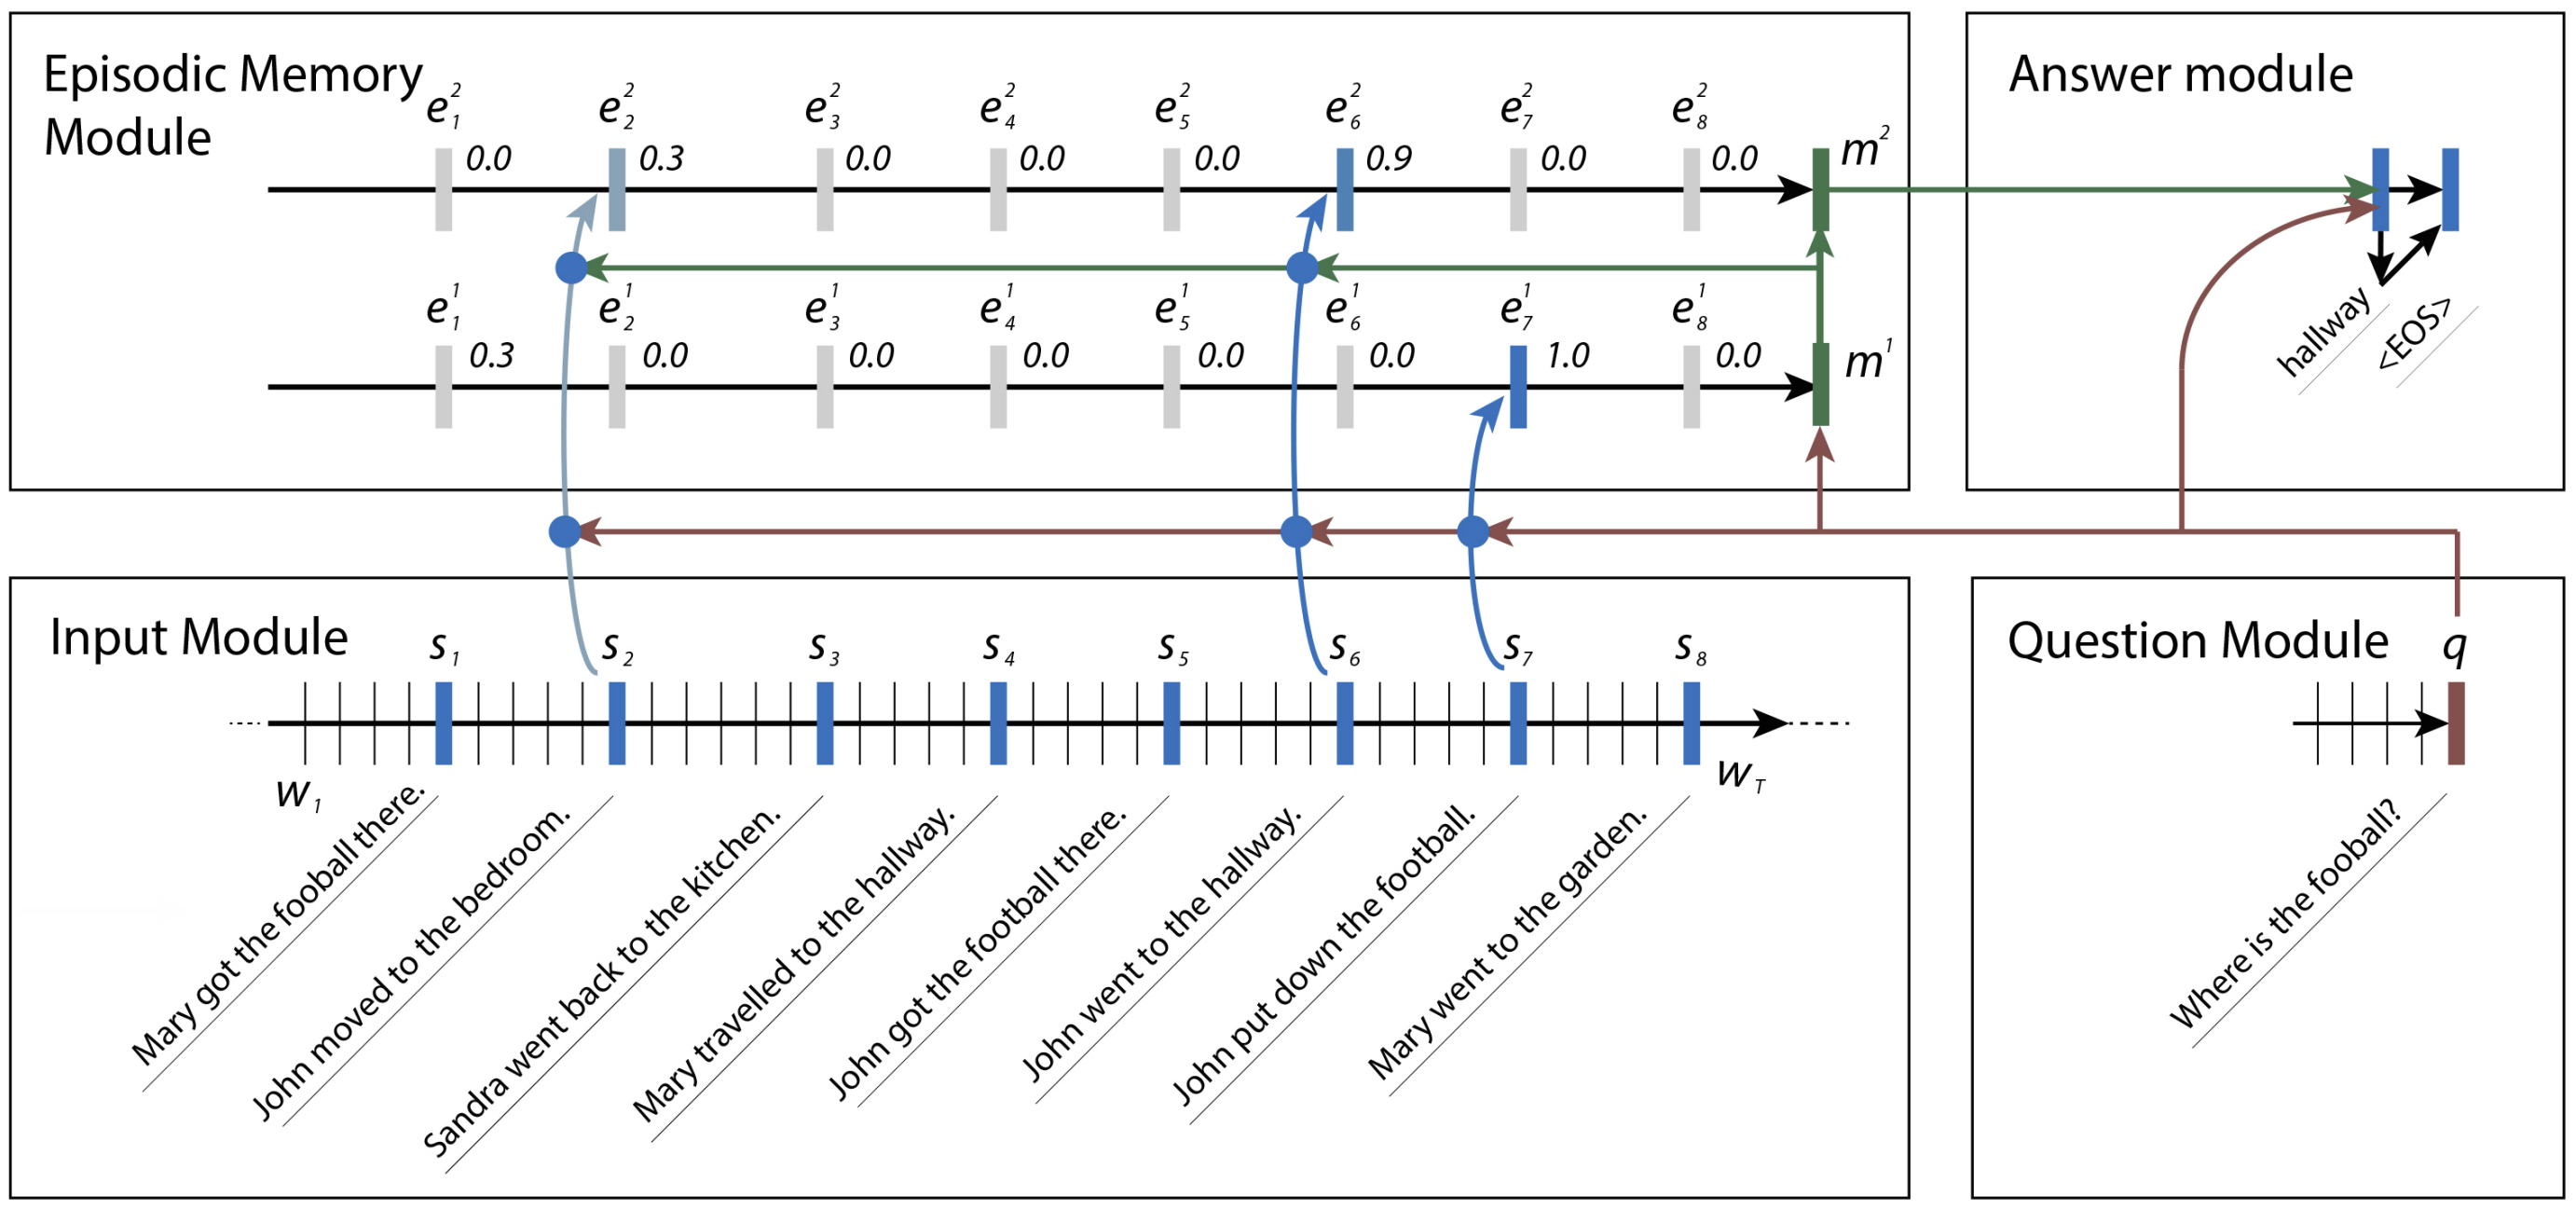
\includegraphics[scale=0.3]{dmn_arch.png}
\caption{The various modules of the DMN. The semantic memory module is not shown, but conceptually it feeds into the input module.}\label{dmn_arch}
\end{figure}

\subsubsection{Episodic memory module}
As mentioned earlier, the episodic memory module consists of a series of modified GRUs, each one attending over the input module's output using the final hidden state of the previous GRU and the question mo. The number of these stacked GRUs (each one essentially being another pass over the input) can either be fixed, or you can use a classifier at the end of each one to decide whether to do another pass.

The main mechanism of the GRU is governed by the following equation:
$$h_i^t = g_i^t\text{GRU}\left(c_i, h_{i-1}^t\right) + (1 - g_i^t)h_{i-1}^t,$$
where $t$ represents which pass over the input we're on, $i$ represents the position in the sequence, $c_i$ is the $i$-th item in the input module's output, $h_i^t$ represents the hidden units, and $g_i^t$ represents the attention mechanism. $g_i^t$ is calculated as:
\begin{align*}
z_i^t &= \left[c_i \circ q; c_i \circ m^{t-1}; \left| c_i - q\right|; \left| c_i - m^{t-1}\right|\right]\\
Z_i^t &= W^{(2)}\tanh\left(W^{(1)}z_i^t + b^{(1)}\right) + b^{(2)}\\
g_i^t &= \frac{\exp\left(Z_i^t\right)}{\sum_i \exp\left(Z_i^t\right)}\\
\end{align*}
Here $\circ$ denotes elementwise multiplication and $|x|$ denotes absolute value. $m^{t}$ denotes the final hidden state of the $t$-th GRU, $W^{(1)}$ and $W^{(2)}$ are learned weight matrices, and $b^{(1)}$ and $b^{(2)}$ are learned bias vectors. Intuitively, $g_i^t$ is activated when the current $c_i$ is determined to be important to answering the question.

A similar model to the DMN is the Memory Network (\begin{tt}https://arxiv.org/pdf/1410.3916.pdf\end{tt}). Some points of comparison:
\begin{itemize} 
\item Both have input, scoring, attention/response mechanisms.
\item MemNets use bag-of-words representation of inputs and explicitly encodes position into embeddings.
\item MemNets iteratively run many different kinds of functions, including for attention and response. (In contrast, the DMN mostly runs on GRUs.)
\end{itemize}
The papers (MemNets linked above, DMNs at beginning) offer more details.

\subsection{Results}
The model performed comparably to the existing state-of-the-art on the bAbI dataset tasks, and achieved new state-of-the-art on the Stanford Sentiment Treebank dataset (sentiment analysis) and matched the existing state-of-theart on POS tagging (WSJ-PTB dataset, on which it actually achieved new state-of-the-art by ensembling the 4 best dev-tuned models). Interestingly, the results showed that the optimal number of passes to perform over the input differed with each task (e.g. 2 for sentiment analysis and 5 for 3-fact reasoning).

It's interesting to examine some examples on the sentiment analysis dataset where the DMN predicted the wrong answer when only given one pass over the input, but got the correct answer when given two passes:
\begin{itemize}
\item ``In its ragged, cheap, and unassuming way, the movie works.” (Answer: positive, one-pass predicted negative)
\item ``The best way to hope for any chance of enjoying this film is by lowering your expectations.” (Answer: negative, one-pass predicted very positive)
\item ``The film starts out as competent but unremarkable…and gradually grows into something of considerable power.” (Answer: positive, one-pass predicted negative)
\item ``My response to the film is best described as lukewarm.” (Answer: negative, one-pass predicted positive)
\end{itemize}

For POS tagging, the model put the answer module on every sequence position, and also only performed one pass over the input.

\subsubsection{Image question answering?}
A subsequent paper (\begin{tt}https://arxiv.org/abs/1603.01417\end{tt}) replaced the input module of the DMN with a CNN that extracted features from images, and was able to achieve new state-of-the-art results on the Visual Question Answering dataset. At an extremely high level, the CNN extracted a $14\times 14$ grid of 512-dimensional feature vectors from each image and passed those into a bidirectional GRU in the input module.

\section{Lecture 17: Issues in NLP and Possible Architectures for NLP}
This lecture is mostly a hodge-podge of various different topics.
\subsection{Solving Language}
As of this lecture (early 2017), a lot of deep learning experts (Yann LeCun, Geoffrey Hinton, etc.) are out to ``solve" NLP in a way like ImageNet ``solved" computer vision. (As of March 2019, which is when I'm drafting these notes for the first time, the Transformer architecture may be able to make that claim.) For a few years prior, the research community had been content to just run LSTMs and get incremental improvements, even though researchers had much more lofty goals in the 1980s, despite realities being much more modest.

In Peter Norvig's 1986 dissertation, he mentioned that, for an NLP system, ``...a suitable knowledge base is a prerequisite for making proper inferences”. We now know that's not true, but the types of inferences he was talking about are still educational. He discussed 4 basic types of inference (as well as two more that were combinations of these 4):
\begin{itemize}
\item Elaboration: filling in a slot to connect two entities, usually with a reason. Example: John had a piggybank REASON to have money REASON to buy a present.
\item Coreference resolution (see Lecture 15)
\item View application, e.g. metaphor interpretation. For example, if I say ``The Red Sox killed the Yankees," I mean that the Red Sox soundly defeated the Yankees in a baseball match, not that they literally murdered the members of the opposing team.
\item Concretization, or inferring a more specific description from a general one. For example, if it's mentioned that I traveled somewhere alone in a (non-autonomous) car, it can be inferred that I drove there.
\end{itemize}
Obviously we've made a ton of progress since 1986. One example of an area that's much better today is syntactic parsing - Norvig actually mentioned in his dissertation the difficulties of using PHRAN (a syntactic parsing program of the time) to parse sentences, but modern systems are able to do it quite well. However, we haven't really gotten good at all four of his tasks; elaboration, for example, is still very hard with modern systems.

So what's the state of NLP as of early 2017?
\begin{itemize}
\item Bidirectional LSTMs with attention are improving state of the art on pretty much every task. (As of early 2019 Transformers seem to be doing the same thing.)
\item Neural methods are leading to a text generation renaissance - they're doing way better than previous methods and improvements are happening very quickly.
\item The question is being raised of whether we need to work with explicit localist language representations (like syntactic structures and semantic frames) at all in complex NLP tasks. For example, DMNs (see Lecture 16) do away with all of this and perform quite well.
\end{itemize}
But obviously there are still areas with lots of work to be done:
\begin{itemize}
\item Methods for building memory/knowledge bases are pretty primitive. LSTMs can remember 100 words or so, but no model is able to accumulate years worth of knowledge and experience like a human brain.
\item Our models aren't good at understanding inter-sentence relationships.
\item Our models can't produce elaborations from a situation using common-sense knowledge.
\end{itemize}

\subsection{Tree RNNs revisited}
See Lecture 14 for the first introduction to tree RNNs.

Tree RNNs are a very theoretically appealing structure - they take advantage of recursion, which is a fundamental aspect of (almost) all languages. They've also been shown to perform competitively in practice. However, they're computationally slow, are often used with an external model to parse syntactic structure, and commonly fail to take advantage of the complementary linear structure of language. 

Note: The reason that tree RNNs are computationally slow compared to LSTMs is because they have a hard time exploting the batch parallelization that GPUs are capable of. In an LSTM, you're guaranteed that every sentence in a batch follows the same pattern of computation (a fixed sequence). However, because each sentence might be structured differently when using a tree RNN model, this falls apart when using tree RNNs, and GPUs are not really able to batch-process multiple sentences at a time. (I'm not completely sure on the technical details here, but I think this is the general idea.)

\subsubsection{SPINN}

The Shift-reduce Parser-Interpreter Neural Network (SPINN) model (\begin{tt}https://arxiv.org/abs/1603.06021 \end{tt}) attempts to address all three of these difficulties. It improves batch processing efficiency, operates standalone (without an external parser), and operates linearly over sentences. 

A beginning observation that motivated this model is that every tree structure can be represented as a sequence of SHIFT and REDUCE, where SHIFT takes a word from the buffer and puts it on the stack, and REDUCE combines the top two elements on the stack into a single element (see Lecture 6 for how the buffer and stack work). For example, the representation (I (eat bread)) of the sentence ``I eat bread" can be represented as SHIFT SHIFT SHIFT REDUCE REDUCE.

The model can basically be described as two parts: a tracking LSTM (with a stack and buffer) and a compositional tree RNN. The LSTM takes in the top element of the buffer and the top two elements of the stack as inputs, and at each time step decides to either SHIFT (move the element on top of the buffer onto the top of the stack) or REDUCE (pop the top two elements off the stack, compose them with the tree RNN, and place the result back on the stack).

The authors had to do some tricks to implement the stack efficiently - if they implemented it naively, it would have run into the same computational issues that tree RNNs historically had. Instead, when the top two elements on the stack were composed, they were not popped off - the composition was simply pushed onto the stack on top of its two children. Structure was maintained by keeping a list of backpointers, which was a sorted list of which elements were actually in the stack. (For example, if we started with a stack of 3 elements with no compositions, the backpointers would simply be (1, 2, 3). If we composed the top two elements, the stack would now have 4 elements, and the backpointers would be (1, 4), since elements 2 and 3 were composed and no longer actually in the stack.)

SPINN was able to achieve new state-of-the-art on the Stanford Natural Language Inference dataset, where the task is to predict an entailment, contradiction, or neutral relationship between two sentences. On this task, SPINN was used to independently generate a ``meaning" vector for each of the two sentences, and those vectors were then fed to a simple feedforward neural network to perform classification. Some examples of cases where SPINN edged out the previous best (an LSTM model) were sentences involving negation, where word order or a single additional word can flip the meaning of the sentence, and sentences that were very long (\textgreater 20 words).

\subsection{Out-of-vocabulary}
New and rare out-of-vocabulary words are an issue with pretty much all NLP tasks. In tasks that involve generating a target text from some source text (e.g. machine translation, question answering), these words are difficult to interpret when encountered in the source, and difficult to generate in the target. One model attempted to address this issue in these types of tasks by training a classifier with the decoder that would decide whether to choose a word from the vocabulary (using softmax) or copy over a word from the input. (Paper: \begin{tt}https://arxiv.org/abs/1603.08148\end{tt}.) This is sometimes referred to as a pointer/copying model. However, another method has been gaining traction as of this lecture.

\subsubsection{Sub-word models}
Before getting into the details of sub-word models, it's worth motivating why they may be helpful.

Most deep learning NLP starts by looking at written language, since it's easily processed and there's a lot of data available. However, not all writing systems are the same:
\begin{itemize}
\item Some systems are phonemic (where basically each phoneme is written down, e.g. Italian)
\item Fossilized phonemic (where the written form indicates phonemes, but isn't a perfect mapping, e.g. English)
\item Syllabic/moraic (each unit of writing is one syllable, and units can be broken down into subunits that indicate phonemes, e.g. Korean)
\item Ideographic (syllabic, but each syllable's symbol doesn't really indicate phonemes in its sub-parts, e.g. Chinese)
\item A mixture of the above (e.g. Japanese)
\end{itemize}
Word representations also vary a lot:
\begin{itemize}
\item Some systems (e.g. Chinese) don't delimit words.
\item Some languages keep clitics (e.g. the 'm in I'm) separate, like French, while some combine many of them together, like Arabic.
\item Some languages keep word compounds separate, like English (``life insurance company employee"), while others agglutinate them into a single word, like German (``Lebensversicherungsgesellschaftsangestellter").
\end{itemize}
Thus there is a need for language models that can handle large, open vocabularies. Obviously this can be helpful for languages with rich morphologies that allow morphemes to be combined into words in many different ways, but it can also help with things like informal spellings (``gooooood morning!") and transliteration (e.g. ``John" should not just be copied if translating to Spanish; rather it should be transliterated as ``Juan").

Deep learning hasn't really explored the traditional-linguistics decomposition of words into morphemes (e.g. ((un((fortun)ate))ly) as a decomposition of ``unfortunately"). One alternative that people have tried is by working with character n-grams (Rumelhart \& McClelland 1986; Microsoft DSSM, Huang et al. 2013), which can give the benefits of using morphemes more easily.

One other avenue of exploration that's gotten more attention is character-level modeling. Character embeddings allow word embeddings for unknown words to be generated from character embeddings, which works reasonably well in practice - words with similar spellings share similar embeddings are are likely to actually have similar meaning. An example of a character-based model is this character-level LSTM that achieved state-of-the-art results in POS tagging: \begin{tt}https://arxiv.org/abs/1508.02096\end{tt}. However, it's not obvious that this would have succeeded, as characters aren't really a semantic unit in traditional linguistics. 

An area where sub-word models are getting traction is machine translation. Here models are following two trends:
\begin{itemize}
\item Some models use a similar seq2seq architecture, like this one: \begin{tt}http://www.aclweb.org/anthology/P16-1162\end{tt}.
\begin{itemize}
\item The key idea behind this paper is a compression algorithm called byte-pair encoding, where a sequence of bytes is compressed by repeatedly taking the most common byte pair (``bigram") and assigning a single (previously unused) byte to map to that byte pair. 
\item The authors used this idea to generate a vocabulary of some predetermined size (say 30k), starting from unigrams, and then repeatedly taking the most common n-gram that doesn't yet have a vocabulary item as a new vocabulary item. This automatically generates a vocabulary from a corpus.
\item Google's machine translation (as of the lecture) does something similar: they use a wordpiece model, but wordpieces are chosen using a greedy algorithm that approximately maximizes language model log likelihood.
\end{itemize}
\item Other models use a hybrid approach, using a word-level RNN where possible, and a separate character-level model elsewhere. An example is \begin{tt}https://arxiv.org/abs/1604.00788\end{tt}.
\begin{itemize}
\item The advantage of mostly operating at the word level is that it is faster than operating at the character level. 
\item At its core, this model has a word-level encoder-decoder machine translation system operating over a fixed vocabulary. Its innovation lies in how it deals with out-of-vocabulary words.
\begin{itemize}
\item When an OOV word occurs in the input, it generates an embedding for it using a character-level LSTM.
\item At decoding time, the model may produce a special UNK token, indicating an unknown word. When this happens, it takes the hidden state of the word-level RNN as the initial input for a character-level LSTM and generates an output word. One detail is that the embedding of this output word is not fed back into the decoder at the next time step as would be customary for other output words; instead, we just feed UNK back into the decoder as the previous output. (This is done for performance reasons.)
\end{itemize}
\item During decoding, the model performs beam search at both the word level and the character level.
\item This model was able to achieve state-of-the-art results on English-Czech translation. Czech has a relatively rich morphology, so previous models were often getting stuck on OOV words or doing inappropriate point-and-copy (e.g. copying ``11-year-old", when it should have been translated to an actual word).
\end{itemize}
\end{itemize}

\end{document}
